\documentclass[a4paper,10pt]{article}
\usepackage{geometry,gretlhds}
\usepackage{url,fancyvrb}
\usepackage{pifont}
\usepackage[utf8]{inputenc}
\usepackage{graphicx}
\usepackage[authoryear]{natbib}
\usepackage{color}
\usepackage{dcolumn,amsmath,mathrsfs}

\newenvironment{funcdoc}[1]
{\noindent\hrulefill\newline\nopagebreak\texttt{#1}%
\nopagebreak\par\noindent\hrulefill%
\nopagebreak\par\nopagebreak\smallskip\nopagebreak\par}
{\bigskip}

% ---------- Ripped from gretl.sty ----------------------------------------

\newcommand{\scriptname}{Example}

\newcommand{\app}[1]{\textsf{#1}}
\newcommand{\cmd}[1]{\texttt{#1}}
\newcommand{\varname}[1]{\texttt{#1}}
\newcommand{\option}[1]{\texttt{-{}-#1}}
\newcommand{\ttsl}[1]{\ttfamily{\textsl{#1}}\normalfont}

\newenvironment{textcode}{\par\small\ttfamily}
{\normalfont\normalsize\par}

\DefineVerbatimEnvironment%
{code}{Verbatim}
{fontsize=\small, xleftmargin=1em}

\DefineVerbatimEnvironment%
{scode}{Verbatim}
{frame=lines, framesep=2ex, fontsize=\footnotesize,
 formatcom=\color{myteal}, rulecolor=\color{mygray}}

\DefineVerbatimEnvironment%
{scodebit}{Verbatim}
{fontsize=\small, formatcom=\color{myteal}}

\DefineVerbatimEnvironment%
{scodebot}{Verbatim}
{frame=bottomline, framesep=2ex, fontsize=\small,
 formatcom=\color{myteal}, rulecolor=\color{mygray}}

\renewcommand{\arraystretch}{1.2}

\definecolor{mygray}{rgb}{0.85,0.85,0.85} 
\definecolor{myteal}{rgb}{0.0,0.25,0.15} 

\def\floatpagefraction{.8}

%% add script as float (Example)
\newcounter{script}[section]
\renewcommand \thescript
     {\ifnum \c@chapter>\z@ \thechapter.\fi \@arabic\c@script}
\def\fps@script{tbp}
\def\ftype@script{1}
\def\ext@script{los}
\def\fnum@script{\scriptname\nobreakspace\thescript}
\newenvironment{script}
               {\@float{script}}
               {\end@float}
\newenvironment{script*}
               {\@dblfloat{script}}
               {\end@dblfloat}
\newcommand\theHscript{\thechapter.\arabic{script}}

\bibliographystyle{apalike}
% ---------- End rip ------------------------------------------------------

\newcommand{\PrE}[1]{\ensuremath \varepsilon_{#1}}
\newcommand{\StS}[1]{\ensuremath u_{#1}}
\newcommand{\InfSet}[1]{\ensuremath \mathcal{F}_{#1}}
\newcommand{\VarSym}{\ensuremath \Phi}
\newcommand{\IRF}[1]{\ensuremath \mathcal{I}_{#1}}
\newcommand{\FEVD}[1]{\ensuremath \mathcal{VD}_{#1}}
\newcommand{\pder}[2]{\ensuremath\frac{\partial #1}{\partial #2}}
\DeclareMathOperator{\VEC}{\mathrm{vec}}
\newlength{\irfw}
\newlength{\irfh}
\setlength{\irfw}{6.5cm}
\setlength{\irfh}{30mm}
\newcommand{\rk}[1]{\mathrm{rank}\left(#1\right)}

\title{The SVAR addon for \app{gretl}}
\author{Jack Lucchetti}
\date{Version 1.2}
\begin{document}

\maketitle

% \begin{abstract}
%   Here we discuss how to estimate Structural VARs (SVARs) in
%   \texttt{gretl} via the \texttt{SVAR} package. 
% \end{abstract}


\tableofcontents

\clearpage

\section{Introduction}
\label{sec:intro}

The \texttt{SVAR} package is a collection of \app{gretl} scripts to
estimate Structural VARs, or SVARs for short. 

In the remainder of this guide, the emphasis will be put on the
scripting interface, which is the recommended way of using the
package. However, most, if not all, of its features are also
accessible via the ``Structural VAR'' menu entry (go to \emph{Model
  $>$ Time Series}) and the corresponding menu-driven interface. The
impatient reader, who already has some understanding of what a SVAR is
and is looking for a step-by-step guide on how to get her work done
quickly via point-and click methods, can consult section \ref{sec:GUI}
in the Appendix.

% (Jack, I upgraded the GUI subsec to a section on purpose.)
In order to establish notation and define a few concepts, allow me to
inflict on you a 2-page crash course on SVARs.  In this
context,\footnote{The adjective ``structural'' is possibly one of the
  most widely used and abused in econometrics. In other contexts, it
  takes a totally different, and unrelated, meaning.} we call
``structural'' a model in which we assume that the one-step-ahead
prediction errors $\PrE{t}$ from a statistical model can be thought of
as linear functions of the \emph{structural shocks} $\StS{t}$. In its
most general form, a structural model is the pair of equations
\begin{eqnarray}
  \label{eq:one-step-ahead}
  \PrE{t} & = & y_t - E(y_t | \InfSet{t-1}) \\
  \label{eq:PrE-StS-AB}
  A \PrE{t} & = & B \StS{t}
\end{eqnarray}
where $\InfSet{t-1}$ is the information set at $t-1$.

In practically all cases, the statistical model is a a finite-order
VAR and equation \eqref{eq:one-step-ahead} specialises to
\begin{equation}
  \label{eq:VAR}
  y_t = \mu' x_t + \sum_{i=1}^p \VarSym_i y_{t-i} + \PrE{t}
  \qquad\mathrm{or}\qquad
  \VarSym(L) y_t = \mu' x_t + \PrE{t}
\end{equation}
where the VAR may include an exogenous component $x_t$, which
typically contains at least a constant term. The above model is
referred to as the AB-model in Amisano-Giannini (1997).

The object of estimation are the square matrices $A$ and $B$;
estimation is carried out by maximum likelihood. After defining $C$ as
$A^{-1}B$, the relationship between prediction errors and structural
shocks becomes
\begin{equation}
  \label{eq:PrE-StS-C}
  \PrE{t} = C \StS{t}
\end{equation}
and under the assumption of normality the average log-likelihood can
be written as
\[
  \mathcal{L} = \mathrm{const} - \ln |C| - 0.5 \cdot
  \mathrm{tr}(\hat{\Sigma} (CC')^{-1}) 
\]

As is well known, the above model is under-identified and in order for
the log-likelihood to have a (locally) unique maximum, it is necessary
to impose some restrictions on the matrices $A$ and $B$. This issue
will be more thoroughly discussed in section \ref{sec:SVARid}; for the
moment, let's just say that some the elements in $A$ and $B$ have to
be fixed to pre-specified values. The minimum number of restrictions
is $n^2 + \frac{n^2 - n}{2}$. This, however, is a necessary condition,
but not sufficient by itself.

The popular case in which $A=I$ is called a C-model. Further, a
special case of the C-model occurs when $B$ is assumed to be
lower-triangular. This was \citeauthor{sims80}'s (\citeyear{sims80})
original proposal, and is sometimes called a ``recursive''
identification scheme. It has a number of interesting properties,
among which the fact that the ML estimator of $C$ is just the Cholesky
decomposition of $\hat{\Sigma}$, the sample covariance matrix of VAR
residuals. This is why many practitioners, including myself, often use
the ``recursive model'' and ``Cholesky model'' phrases
interchangeably.  This has been the most frequently used variant of a
SVAR model, partly for its ease of interpretation, partly for its ease
of estimation.\footnote{Some may say ``partly for the unimaginative
  nature of applied economists, who prefer to play safe and maximise
  the chances their paper isn't rejected rather than risk and be
  daring and creative''. But who are we to judge?} In the remainder of
this document, a lower-triangular C model will be called a ``plain''
SVAR model.

If the model is just-identified, $\hat{\Sigma} (CC')^{-1}$ will be the
identity matrix and the log-likelihood simplifies to
\[
  \mathcal{L} = \mathrm{const} - 0.5 \ln |\hat{\Sigma}| - 0.5 n
\]
Of course, it is possible to estimate constrained models by imposing
some extra restrictions; this makes it possible to test the
over-identifying restrictions easily by means of a LR test.

Except for trivial cases, like the Cholesky decomposition,
maximisation of the likelihood involves numerical
iterations. Fortunately, analytical expressions for the score, the
Hessian and the information matrix are available, which helps a
lot;\footnote{As advocated in \citeauthor{AG}, the scoring algorithm
  is used by default, but several alternatives are available. See
  subsection \ref{sec:algorithms} below.} once convergence has
occurred, the covariance matrix for the unrestricted elements of $A$
and $B$ is easily computed via the information matrix.

Once estimation is completed, $\hat{A}$ and $\hat{B}$ can be used to
compute the structural VMA representation of the VAR, which is the
base ingredient for most of the subsequent analysis, such as Impulse
Response Analysis and so forth. If the matrix polynomial $\VarSym(L)$ in
equation \eqref{eq:VAR} is invertible, then (assuming $x_t=0$ for ease of
notation), $y_t$ can be written as
\begin{equation}
  \label{eq:vma}
y_t = \VarSym(L)^{-1}\PrE{t} = \Theta(L) \PrE{t} = \PrE{t} + \Theta_1
\PrE{t-1} + \cdots
\end{equation}
which is known as the VMA representation of the VAR. Note that in
general the matrix polynomial $\Theta(L)$ is of infinite order.

From the above expression, one can write the \emph{structural} VMA
representation as
\begin{equation}
  \label{eq:svma}
  y_t = C \StS{t} + \Theta_1 C \StS{t-1}  + \cdots 
      = M_0 \StS{t} + M_1 \StS{t-1}  + \cdots 
\end{equation}
From equation \eqref{eq:svma} it is immediate to compute the impulse response
functions:
\[
  \IRF{i,j,h} = \pder{y_{i,t}}{\StS{j, t-h}} = \pder{y_{i,t+h}}{\StS{j, t}} 
\]
which in this case equal simply
\[
  \IRF{i,j,h} = \left[ M_h \right]_{ij}
\]
The computation of confidence intervals for impulse responses could,
in principle, be performed analytically by the delta method (see
\cite{Lut90}). However, this has two disadvantages: for a start, it is
quite involved to code. Moreover, the limit distribution has been
shown to be a very poor approximation in finite samples (see for
example \cite{FaBra96} or \cite{Kilian98}), so the bootstrap is almost
universally adopted, although in some cases it may be quite CPU-heavy.

%\pagebreak[4]

\section{C models}
\label{sec:Cmodel}
\subsection{A simple example}

\begin{table}[htbp]
  \label{InternalChol-in}
  \begin{code}
# turn extra output off
set echo off
set messages off

# open the data and do some preliminary transformations
open sw_ch14.gdt
genr infl = 400*ldiff(PUNEW)
rename LHUR unemp
list X = unemp infl

var 3 unemp infl

Sigma = $sigma
C = cholesky(Sigma)
print Sigma C
  \end{code}
%$
  \caption{Cholesky example via the internal \texttt{gretl} command}
\end{table}

As a trivial example, we will estimate a plain Cholesky model. The
data are taken from Stock and Watson's sample data
\texttt{sw\_ch14.gdt}, and our VAR will include inflation and
unemployment, with a constant and 3 lags. Then, we will compute the
IRFs and their 90\% bootstrap confidence interval.\footnote{Why not
  95\%? Well, keeping the number of bootstrap replications low is one
  reason. Anyway, it must be said that in the SVAR literature few
  people use 95\%. 90\%, 84\% or even 66\% are common choices.}

\begin{table}[htbp]
  \label{InternalChol-out}
  \centering
  \begin{code}
VAR system, lag order 3
OLS estimates, observations 1960:1-1999:4 (T = 160)
Log-likelihood = -267.76524
Determinant of covariance matrix = 0.097423416
AIC = 3.5221
BIC = 3.7911
HQC = 3.6313
Portmanteau test: LB(40) = 162.946, df = 148 [0.1896]

Equation 1: u

             coefficient   std. error   t-ratio   p-value 
  --------------------------------------------------------
  const       0.137300     0.0846842     1.621    0.1070  
  u_1         1.56139      0.0792473    19.70     8.07e-44 ***
  u_2        -0.672638     0.140545     -4.786    3.98e-06 ***

...
Sigma (2 x 2)

    0.055341    -0.028325 
   -0.028325       1.7749 

C (2 x 2)

     0.23525       0.0000 
    -0.12041       1.3268 
  \end{code}
  \caption{Cholesky example via the internal \texttt{gretl} command --- Output}
\end{table}

\begin{figure}[htbp]
  \centering
  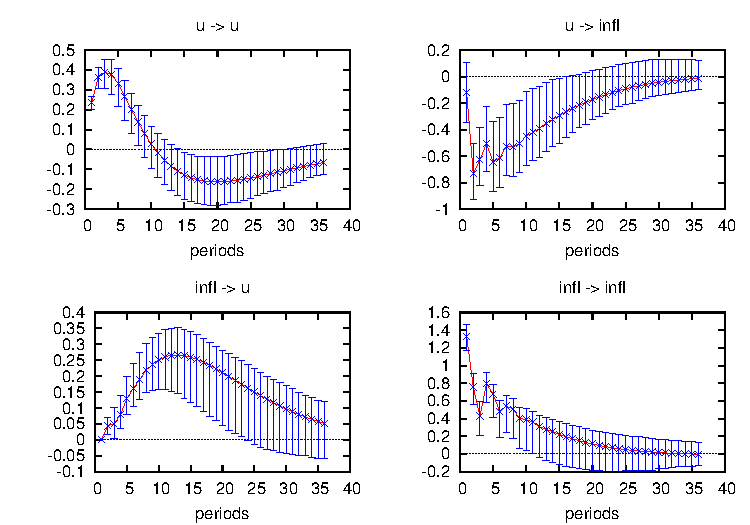
\includegraphics{simpleC_gretl}
  \caption{Impulse response functions for the simple Cholesky model (native)}
  \label{fig:nativeIRF}
\end{figure}

%\subsubsection{Gretl native \texttt{var} command}
In order to accomplish the above, note that we \emph{don't} need to
use the \texttt{SVAR} package, as a Cholesky SVAR can be handled by
\texttt{gretl} natively. In fact, the script shown in Table
\ref{InternalChol-in} does just that: runs a VAR, collects
$\hat{\Sigma}$ and estimates $C$ as its Cholesky decomposition. 
Part of its output is in Table \ref{InternalChol-out}.  The impulse
responses as computed by \texttt{gretl}'s internal command can be see
in figure \ref{fig:nativeIRF}. See the Gretl User's Guide for more
details.

%\clearpage

\subsection{Base estimation via the \texttt{SVAR} package}
\label{sec:baseest}

We will now replicate the above example via the \texttt{SVAR} package;
in order to do so, we need to treat this model as a special case of
the C-model, where $\PrE{t} = C \StS{t}$ and identification is
attained by stipulating that $C$ is lower-triangular, that is

\begin{equation}
  \label{eq:cholesky}
  C = \left[ \begin{array}{ll} 
      c_{11} & 0 \\ c_{12} & c_{22}    
  \end{array} \right].
\end{equation}

\begin{table}[htbp]
\begin{scode}
# turn extra output off
set echo off
set messages off

# open the data and do some preliminary transformations
open sw_ch14.gdt
genr infl = 400*ldiff(PUNEW)
rename LHUR unemp
list X = unemp infl
list Z = const

# load the SVAR package
include SVAR.gfn

# set up the SVAR
Mod = SVAR_setup("C", X, Z, 3)

# Specify the constraints on C
SVAR_restrict(&Mod, "C", 1, 2, 0)

# Estimate
SVAR_estimate(&Mod)
  \end{scode}
  \caption{Simple C-model}
  \label{tab:simpleC-base}
\end{table}

Table \ref{tab:simpleC-base} shows a sample script to estimate the
example Cholesky model: the basic idea is that the model is contained
in a \app{gretl} bundle.\footnote{Bundles are a \app{gretl} data type:
  they may be briefly described as containers in which a certain
  object (a scalar, a matrix and so on) is associated to a ``key'' (a
  string). Technically speaking, a bundle is an associative array:
  these data structures are called ``hashes'' in Perl or
  ``dictionaries'' in Python. Fore more info, you'll want to take a
  look at the Gretl User's Guide, section 11.7.} In this example,
the bundle is called \texttt{Mod}, but it can of course take any valid
\texttt{gretl} identifier.

After performing the same preliminary steps as in the example in Table
\ref{InternalChol-in}, we load the package and use the
\texttt{SVAR\_setup} function, which initialises the model and sets up
a few things. This function takes 4 arguments:
\begin{itemize}
\item a string, with the model type (\texttt{"C"} in this example);
\item a list containing the endogenous variables $y_t$;
\item a list containing the exogenous variables $x_t$ (may be
  \texttt{null});
\item the VAR order $p$.
\end{itemize}

Once the model is set up, you can specify which elements you want to
constrain to achieve identification: in fact, the key ingredient in a
SVAR is the set of constraints we put on the structural
matrices. \texttt{SVAR} handles these restrictions via their implicit
form representation $R \theta = d$.  As an example, the constraints
for the simple case we're considering here can be written in implicit
form as
\[
  R \VEC C = d
\]
where $R = \left[ 0, 0, 1, 0 \right]$ and $d=0$.

There are several ways to constrain a model: for a C model, the $R^* =
[R | d ]$ matrix is stored as the bundle element \texttt{Rd1} and the
number of its rows is kept as bundle element \texttt{nc1}. If you feel
like building the matrix $R^*$ via \app{gretl}'s ordinary matrix
functions, all you have to do is to fill up the bundle elements
\texttt{Rd1} and \texttt{nc1} properly before calling
\texttt{SVAR\_estimate()}.

In most cases, however, you'll want to use the \texttt{SVAR\_restrict}
function, which gives you a much more straightforward tool. A complete
description can be found in appendix \ref{sec:syntax}; suffice it to
say here that the result of the function
\begin{code}
  SVAR_restrict(&Mod, "C", 1, 2, 0)
\end{code}
is to ensure that $C_{1,2} = 0$ (see eq.~\ref{eq:cholesky}). The
\texttt{SVAR\_restrict} function does nothing but add rows to
$R^*$. The function also contains a check so that redundant or
inconsistent restrictions will not be allowed.


The next step is estimation, which is accomplished via the
\texttt{SVAR\_estimate} function, which just takes one argument, the
model to estimate. The output of the \texttt{SVAR\_estimate} function
is shown below:\footnote{For compatibility with other packages,
  $\hat{\Sigma}$ is estimated by dividing the cross-products of the
  VAR residuals by $T-k$ instead of $T$; this means that the actual
  figures will be slightly different from what you would obtain by
  running \texttt{var} and then \texttt{cholesky(\$sigma)}.} note
that, as an added benefit, we get asymptotic standard errors for the
estimated parameters (estimated via the information matrix).

\begin{code}
Unconstrained Sigma:
     0.05676    -0.02905
    -0.02905     1.82044

             coefficient   std. error   z-stat    p-value 
  --------------------------------------------------------
  C[ 1; 1]     0.238243    0.0131548    18.11     2.62e-73 ***
  C[ 2; 1]    -0.121939    0.105142     -1.160    0.2461  
  C[ 1; 2]     0.00000     0.00000      NA       NA       
  C[ 2; 2]     1.34371     0.0741942    18.11     2.62e-73 ***
\end{code}

At this point, the model bundle contains all the quantities that will
need to be accessed later on, including the structural VMA
representation \eqref{eq:svma}, which is stored in a matrix called
\texttt{IRFs} which has $h$ rows and $n^2$ columns. Each row $i$ of
this matrix is $\VEC(M_i)'$, so if you wanted to retrieve the IRF for
variable $m$ with respect to the shock $k$, you'd have to pick its
$[(k-1)\cdot n + m]$-th column.

The number of rows $h$ is called the ``horizon''. The function
\texttt{SVAR\_setup} initialises automatically the horizon to 24 for
monthly data and to 20 for quarterly data. To change it, you just
assign the desired value to the \texttt{horizon} element of the
bundle, as in
\begin{code}
  Mod.horizon = 40
\end{code}
Clearly, this adjustment has to be done \emph{before} the
\texttt{SVAR\_estimate} function is called.
 
More details on the internal organisation of the bundle can be
found in section \ref{sec:bundle_struct} in the appendix. Its contents
can be accessed via the ordinary \app{gretl} syntactic constructs for
dealing with bundles. For example, the number of observations used in
estimating the model is stored as the bundle member \texttt{T}, so
if you ever need it you can just use the syntax \texttt{Mod.T}, or
\texttt{Mod.T}.

Once the model has been estimated, it becomes possible to retrieve
estimates of the structural shocks, via the function
\texttt{GetShocks}, as in:
\begin{code}
  series foo = GetShock(&Mod, 1)
  series bar = GetShock(&Mod, 2)
\end{code}
If we append the two lines above to example \ref{tab:simpleC-base},
two new series will be obtained. The formula used is nothing but
equation \eqref{eq:PrE-StS-C} in which the VAR residuals are used in
place of $\PrE{t}$.

\bigskip

\textbf {Warning:} If you are working on a subsample of your dataset,
keep in mind that the SVAR package follows a different convention than
\app{gretl} for handling the actual start of your sample. Ordinary
\app{gretl} commands, such as \cmd{var}, will use data prior to your
subsampling choice for lags, if present. The SVAR package, on the
contrary, will not. An example should make this clear: suppose your
dataset starts at 1970Q1, but you restrict your sample range only to
start at 1980Q1. The \app{gretl} commands
\begin{code}
  smpl 1980:1 ;
  list X = x y z
  var 6 X
\end{code}
will estimate a VAR with 6 lags, in which the first datapoint for the
dependent variable will be 1980Q1 and data from 1978Q3 to 1979Q4 will
be used for initialising the VAR. However,
\begin{code}
  smpl 1980:1 ;
  list X = x y z
  Model = SVAR_setup("C", X, const, 6)
\end{code}
will estimate the same model on a different dataset: that is, the first
available datapoint for estimation will be 1981Q3 because data from
1980Q1 to 1981Q2 will be needed for lagged values of the $y_t$ variables.

\subsection{Algorithm choice}
\label{sec:algorithms}

Another thing you may want to toggle before calling
\texttt{SVAR\_estimate} is the optimisation method: you do this by
setting the bundle element \texttt{optmeth} to some number between 0
and 4; its meaning is shown below:

\begin{center}
  \begin{tabular}{rl}
    \hline
    \texttt{optmeth} & Algorithm \\
    \hline
	0 & BFGS (numerical score) \\
	1 & BFGS (analytical score) \\
	2 & Newton-Raphson (numerical score) \\
	3 & Newton-Raphson (analytical score) \\
	4 & Scoring algorithm (\textbf{default}) \\
    \hline
  \end{tabular}
\end{center}

So in practice the following code snippet
\begin{code}
  Mod.optmeth = 3
  SVAR_estimate(&Mod)
\end{code}
would estimate the model by using the Newton-Raphson method, computing
the Hessian by numerically differentiating the analytical score. In
most cases, the default choice will be the most efficient; however, it
may happen (especially with heavily over-identified models) that the
scoring algorithm fails to converge. In those cases, there's no
general rule. Experiment!


\subsection{Displaying the Impulse Responses}
\label{sec:IRF-FEVD}

The \texttt{SVAR} package provides a function called \texttt{IRFplot}
for plotting the impulse response function on your screen, with a
little help from our friend \texttt{gnuplot}; its syntax is relatively
simple. \texttt{IRFplot} requires three arguments:
\begin{enumerate}
\item The model bundle (as a pointer);
\item the number of the structural shock we want the IRF to;
\item the number of the variable we want the IRF for.
\end{enumerate}
For example,
\begin{code}
  IRFplot(&Mod, 1, 1)
\end{code}

The function can be used in a more sophisticated way than this (see
later). Its output is presented in Figure
\ref{fig:simpleC-noboot.IRF}. As can be seen, it's very similar to the
one obtained by \texttt{gretl}'s native command (Figure
\ref{fig:nativeIRF}).\footnote{Warning: using the built-in GUI graph
  editor that gretl provides may produce `wrong' results on the
  figures generated by the \texttt{IRFplot} function.  All
  \app{gretl}'s graphics are handled by creating a gnuplot script,
  executing it and then sending the result to the display. All this is
  done transparently. When you edit a graph, you modify the underlying
  gnuplot script via some GUI elements, so when you click ``Apply''
  the graphic gets re-generated. However, \app{gretl}'s GUI interface
  for modifying graphics can't handle arbitrary gnuplot scripts, but
  only those generated internally.

  The figures generated by \texttt{IRFplot} contain a few extra
  features that the GUI editor doesn't handle, so invoking the GUI
  controls may mess up the graph. As an alternative, you can customise
  the graph by editing the gnuplot script directly: right-click on it
  and ``Save [it] to session as icon''. Then, in the icon view, right
  click on the graph icon and choose ``Edit plot commands'': you'll have
  the gnuplot source to the graph, that you can modify as needed.}

\begin{figure}[htbp]
  \centering
    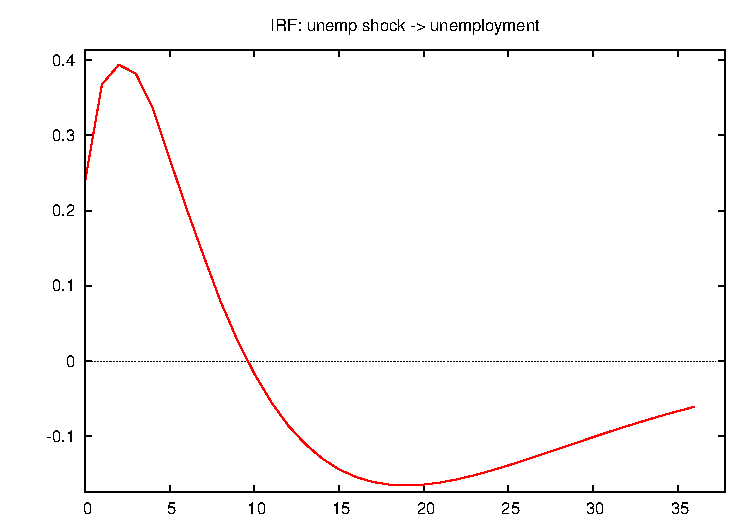
\includegraphics[scale=0.7]{simpleC_11_noboot}
  \caption{Impulse response functions for unemployment}
  \label{fig:simpleC-noboot.IRF}
\end{figure}

By the way: you can attach labels to the structural shocks if you
want. Just store an array of strings with the appropriate number of
elements into the model bundle, under the \texttt{snames} key. For
example,
\begin{code}
  Model.sname = strsplit("foo bar baz")
\end{code}
If you omit this step, the structural shocks will be labelled with
names corresponding to the observable variables in your VAR. This
doesn't make particular sense in general, but it does in a triangular
model, in which there is a one-to-one correspondence, so I decided to
make this the default choice.

\subsection{Bootstrapping}
\label{sec:bootstrap}

\begin{table}[htbp]
\begin{scode}
  bfail = SVAR_boot(&Mod, 1024, 0.90)

  loop for i=1..2 -q
      loop for j=1..2 -q
          sprintf fnam "simpleC_%d%d.pdf", i, j
          IRFsave(fnam, &Mod, i, j)
      end loop
  end loop
  \end{scode}
  \caption{Simple C-model (continued)}
  \label{tab:simpleC-IRF}
%$
\end{table}

The next step is computing bootstrap-based confidence intervals for
the estimated coefficients and, more interestingly, for the impulse
responses: as can be seen in Table \ref{tab:simpleC-IRF}, this task is
given to the \texttt{SVAR\_boot} function, which takes as arguments
\begin{enumerate}
\item The model bundle pointer;
\item the required number of bootstrap replications (1024
  here);\footnote{There's a hard limit at 16384 at the moment;
    probably, it will be raised in the future. However, unless your
    model is very simple, anything more than that is likely to take
    forever and melt your CPU.}
\item the desired size of the confidence interval $\alpha$.
\end{enumerate}

The function outputs a scalar, which keeps track of how many bootstrap
replications failed to converge (none here). Note that this procedure
may be quite CPU-intensive. The output contains a table similar to the
output to \texttt{Cmodel}, which is used to display the bootstrap
means and standard errors of the parameters:
\begin{code}
Bootstrap results (1024 replications)
             coefficient   std. error      z       p-value 
  ---------------------------------------------------------
  C[ 1; 1]     0.232146    0.0183337    12.66      9.57e-37 ***
  C[ 2; 1]    -0.114610    0.143686     -0.7976    0.4251  
  C[ 1; 2]     0.00000     0.00000      NA        NA       
  C[ 2; 2]     1.30234     0.0853908    15.25      1.61e-52 ***

Failed = 0, Time (bootstrap) = 20.24
\end{code}

Once the bootstrap is done, its results are stored into the bundle for
later use: upon successful completion, the model bundle will
contain a bundle\footnote{Yes, bundles can contain bundles.} called
\texttt{bootdata}. This contains some information on the bootstrap
details, such as the confidence interval $\alpha$ and others; in
addition, it will contain three matrices in which each column is one
of the $n^2$ IRFs, and the rows contain
\begin{enumerate}
\item the lower limit of the confidence interval in the
  \texttt{lo\_cb} matrix;
\item the upper limit of the confidence interval in the
  \texttt{hi\_cb} matrix;
\item the medians in the \texttt{mdns} matrix.
\end{enumerate}
where $h$ is the IRF horizon.

In practice, the bootstrap results may be retrieved as follows (the
medians in this example):
\begin{code}
  bfail = SVAR_boot(&Mod, 1024, 0.90)
  scalar h = Mod.horizon
  bundle m = Mod.bootdata
  matrix medians = m.mdns
\end{code}

However, if you invoke \texttt{IRFplot()} after the bootstrap, the
above information will be automatically used for generating the
graph. In this case, you may supply \texttt{IRFplot()} with a fourth
argument, an integer from 0 to 2, to place the legend to the right of
the plot (value: 1), below it (value: 2) or omit it altogether (value:
0). The default, which applies if you omit the parameter, is 1.

Another \texttt{SVAR} function, \texttt{IRFsave()}, is used to
store plots the impulse responses into graphic files files for later
use;\footnote{The format is dictated by the extension you use for the
  output file name: since this job is delegated to \texttt{gnuplot},
  all graphical formats that \texttt{gnuplot} supports are available,
  including pdf, PostScript (via the extension \texttt{ps}), PNG (via
  the extension \texttt{png}) or Scalable Vector Graphics (via the
  extension \texttt{svg}). } its arguments are the same as
\texttt{IRFplot()}, except that the first argument must contain a
valid filename to save the plot into. In the above example, this
function is used within a loop to save all impulse responses in one
go. The output is shown in Figure \ref{fig:simpleC.IRF}.

\begin{figure}[htbp]
  \centering
  \begin{tabular}{cc}
    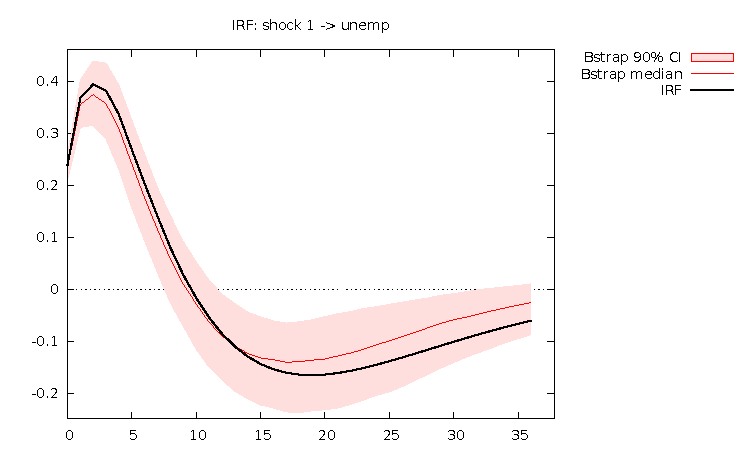
\includegraphics[width=\irfw, height=\irfh]{simpleC_11} &
    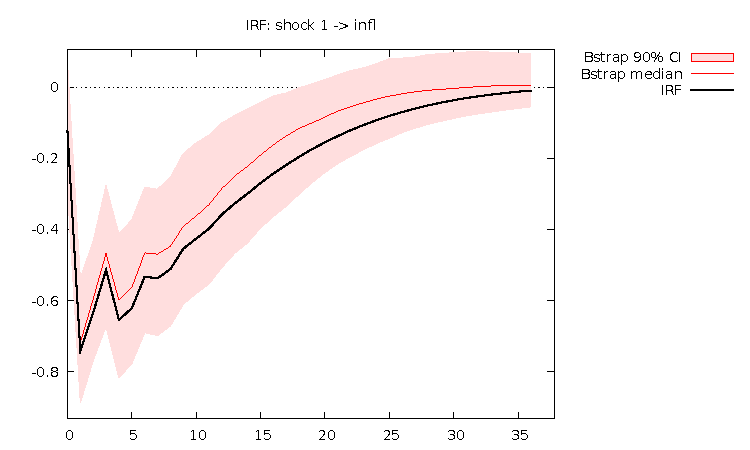
\includegraphics[width=\irfw, height=\irfh]{simpleC_12} \\
    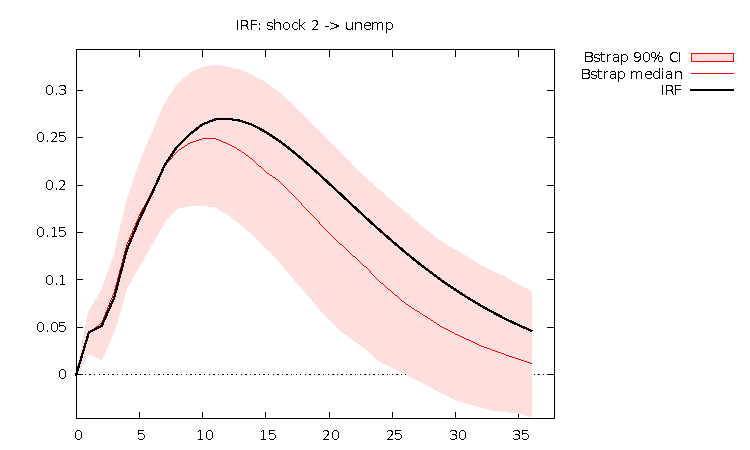
\includegraphics[width=\irfw, height=\irfh]{simpleC_21} &
    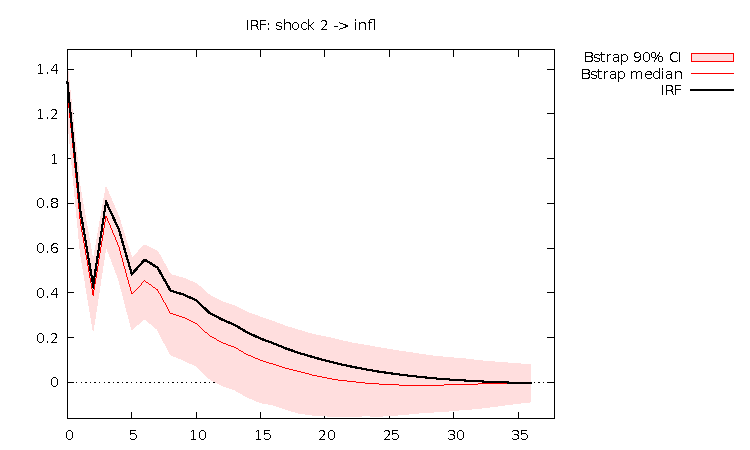
\includegraphics[width=\irfw, height=\irfh]{simpleC_22}
  \end{tabular}
  \caption{Impulse response functions for the simple Cholesky model}
  \label{fig:simpleC.IRF}
\end{figure}

The default method for performing the bootstrap is the the most
straightforward residual-based bootstrap, that is the one put forward
by \cite{Runkle87}. 


As an alternative, one may use bias-correction, which comes in two
flavors, both inspired to the procedure known as
``bootstrap-after-bootstrap'' \citep{Kilian98}.\footnote{None of the
  fancier alternatives listed, for example, in \cite{Brug06} are
  available. They are planned, though.}

The one which corresponds more closely to \citeauthor{Kilian98}'s
proceudre is what what we call the ``Full'' variant; The ``Partial''
variant applies the bias correction only for adjusting the VAR
coefficients used for generating the bootstrap replications, but
\emph{not} for computing the VMA representation. The interested user
may want to experiment with both. 

The ``Partial'' and ``Full'' variant may be enabled by setting the
bundle member \texttt{biascorr} to 1 and 2, respectively, before
calling \texttt{SVAR\_boot}. For an example, look at the example file
\texttt{bias\_correction.inp}.

Finally: if you change the \texttt{optmeth} bundle element before
\texttt{SVAR\_boot} is called, the choice affects the estimation of
the bootstrap artificial models. Hence, you may use one method for the
real data and another method for the bootstrap, if you so desire.

\subsection{A shortcut}

In many cases, a triangular, Cholesky-style specification for the $C$
matrix like the one analysed in this section is all that is
needed. When many variables are involved, the setting of the $\frac{n
  \times (n-1)}{2}$ restrictions via the \texttt{SVAR\_restrict}
function could be quite boring, although easily done via a loop.

For these cases, the \texttt{SVAR} package provides an alternative
way: if you supply the \texttt{SVAR\_setup} function with the string
\texttt{"plain"} as its first argument, the necessary restrictions are
set up automatically. Thus, the example considered above in Table
\ref{tab:simpleC-base} could by modified by replacing the lines
\begin{code}
Mod = SVAR_setup("C", X, Z, 3)
SVAR_restrict(&Mod, "C", 1, 2, 0)
\end{code}
with the one-liner
\begin{code}
Mod = SVAR_setup("plain", X, Z, 3)
\end{code}
and leaving the rest unchanged. Of course, when you have two
variables, such as in this case, there's not much difference, but for
larger systems the latter syntax is much more convenient.

Another advantage is that, in this case, the solution to the
likelihood maximisation problem is known analytically, so no numerical
optimisation technique is used at all. This makes computations much
faster, and for example allows you to make extravagant choices on, for
example, the number of bootstrap replications. Hence, if your C model
can be rearranged as a plain triangular model, it is highly advisable
to do so.

\section{More on plotting}
\label{sec:moreplots}

Traditionally, analysis of the Impulse Response Functions has been the
main object of interest in the applied SVAR literature, but is by no
means the only one.  After estimation, two more techniques are readily
available for inspecting the results: the Forecast Error Variance
Decomposition and the Historical Decomposition. Since the results from
these two procedures are often visualised as graphs, I will describe
them here.

\subsection{Plotting the FEVD}
\label{sec:fevdplots}

Another quantity of interest that may be computed from the structural
VMA representation is the Forecast Error Variance Decomposition
(FEVD).  Suppose we want to predict the future path of the observable
variables $h$ steps ahead, on the basis of the information set
$\InfSet{t-1}$. From equations \eqref{eq:vma} and \eqref{eq:svma} one
obtains that
\[
y_{t+h} - \hat{y}_{t+h} = \sum_{k=0}^h \Theta_k E(\PrE{t+h-k}) =
\sum_{k=0}^h M_k E(\StS{t+h-k})
\]

Since $E(\StS{t+h-k}) = I$ by definition, the forecast error variance
after $h$ steps is given by
\[
  \Omega_h = \sum_{k=0}^h M_k M_k'
\]
hence the variance for variable $i$ is
\[
  \omega^2_i = \left[ \Omega_h \right]_{i,i} = \sum_{k=0}^h e_i' M_k M_k' e_i =
  \sum_{k=0}^h \sum_{l=1}^n ({}_km_{i.l})^2 
\]
where $e_i$ is the $i$-th selection vector,\footnote{That is, a vector
  with zeros everywhere except for a 1 at the $i$-th element.} so
${}_km_{i.l}$ is, trivially, the $i,l$ element of $M_k$. As a
consequence, the share of uncertainty on variable $i$ that can be
attributed to the $j$-th shock after $h$ periods equals
\[
  \FEVD{i,j,h} =
  \frac{\sum_{k=0}^h ({}_km_{i.j})^2 }{\sum_{k=0}^h \sum_{l=1}^n
    ({}_km_{i.l})^2 } .
\]

\begin{table}[htbp]
\begin{scode}
  fevdmat = FEVD(&Mod)
  print fevdmat

  FEVDplot(&Mod, 1)
  FEVDplot(&Mod, 2)
  \end{scode}
  \caption{FEVD: computation and output}
  \label{tab:FEVDprint}
\end{table}

As shown in Table \ref{tab:FEVDprint}, after the model has been
estimated, it can be passed to another function called \texttt{FEVD}
to compute the Forecast Error Variance Decomposition, which is
subsequently printed. Its usage is very simple, since it only needs
one input (a pointer to the model bundle); like the \cmd{IRFplot}
function, you can also attach an extra optional parameter at the end
to control the position of the legend.

\begin{figure}[htbp]
  \centering
  \begin{tabular}{cc}
    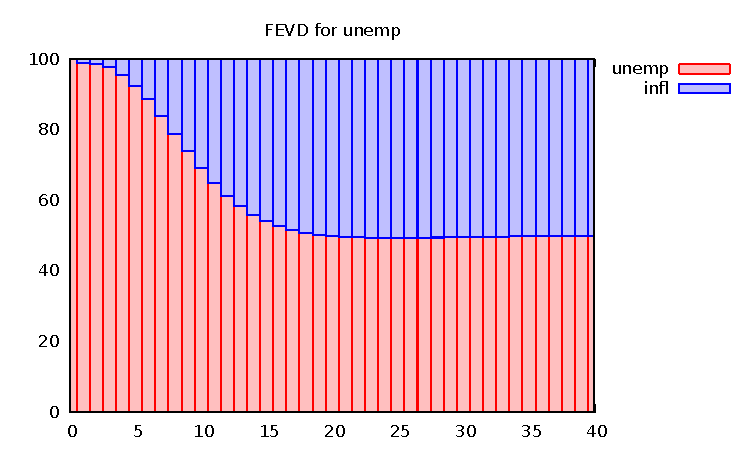
\includegraphics[width=\irfw, height=\irfh]{FEVD_1} &
    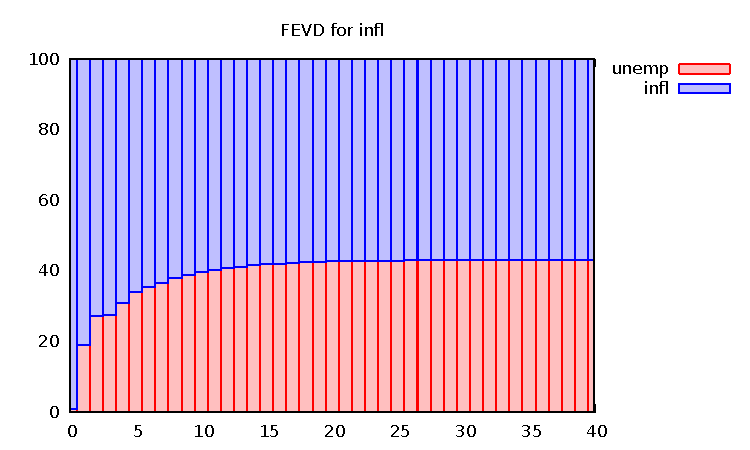
\includegraphics[width=\irfw, height=\irfh]{FEVD_2}
  \end{tabular}
  \caption{FEVD for the simple Cholesky model}
  \label{fig:FEVDplot}
\end{figure}

Since the FEVD for a particular variable is expressed in terms of
shares, it is quite common to depict it graphically as a histogram,
with the horizon on the x-axis. This can be accomplished rather simply
in SVAR by using the specialised function \cmd{FEVDplot()}, which
needs two arguments: a pointer to the model bundle and the number of
the variable you want the FEVD for. Running the code in Table
\ref{tab:FEVDprint} you should see two graphs similar to Figure
\ref{fig:FEVDplot}.

For saving the output to a file, its variant \cmd{FEVDsave()} works
the same, except you need an extra argument (which goes first) with
the filename you choose for the output.\footnote{See also the
  illustration of the \cmd{IRFsave} function at Section
  \ref{sec:bootstrap}.}


\subsection{Historical decomposition}
\label{sec:HD}

\begin{table}[htbp]
\begin{scode}
# turn extra output off
set echo off
set messages off

# open the data and do some preliminary transformations
open sw_ch14.gdt
genr infl = 400*ldiff(PUNEW)
rename LHUR unemp
list X = unemp infl
list Z = const

# load the SVAR package
include SVAR.gfn

# set up the SVAR
Mod = SVAR_setup("C", X, Z, 3)

# Specify the constraints on C
SVAR_restrict(&Mod, "C", 1, 2, 0)

# Estimate
SVAR_estimate(&Mod)

# Save the historical decomposition as a list of series
list HD_infl = SVAR_hd(&Mod, 2)

# Just plot the historical decomposition for unemployment
HDplot(&Mod, 2)
\end{scode}
  \caption{Simple C-model with historical decomposition}
  \label{tab:simpleC-hd}
\end{table}

A natural extension of the FEVD concept (see
sections \ref{sec:intro} and \ref{sec:IRF-FEVD}) is the so-called
\emph{historical decomposition} of observed time series, which can be
briefly described as follows.

Consider the representations \eqref{eq:VAR} and \eqref{eq:svma};
clearly, if one could observe the parameters of the system (the
coefficients of the $\VarSym(\cdot)$ polynomial and the matrix $\mu$) plus
the sequence of structural shocks $\StS{t}$, it would be possible to
decompose the observed path of the $y_t$ variables into $n + 1$
distinct components: first, a purely exogenous one, incorporating the
term $\mu' x_t$ plus all the feedback effects given by the lag
structure $\VarSym(L)$; this is commonly termed the ``deterministic
component'' (call it $d_t$). The remainder $y_t - d_t$ can be
therefore thought of as the superimposition of separate contributions,
given by each structural shock hitting the system at a given time. In
practice, we'd think of each individual series in the system as
\[
 y_{it} - d_{i,t} = M_{i,1}(L) u_{1,t} + \cdots + M_{i,n}(L) u_{n,t} 
\]
using representation \eqref{eq:svma}. 

Note that each element of the sum on the right-hand side of the above
equation is uncorrelated (by hypothesis) of all the other ones at all
leads and lags. Therefore, the contribution of each shock to the
visible path of the variable $y_{it}$ is distinct from the others. In
a way, historical decomposition could be considered as a particular
form of counterfactual analysis: each component $M_{i,j}(L) u_{j,t}$
shows what the history of $y_{i,t}$ would have been if the $j$-th
shock had been the only one affecting the system.

From a technical point of view, the decomposition is computed via a
``rotated'' version of the system:\footnote{I know, I know: strictly
  speaking, it's not a rotation; for it to be a rotation, you ought to
  force $C$ to be orthogonal somehow; but let's not be pedantic, OK?}
pre-multiplying equation \eqref{eq:VAR} by $C^{-1}$ gives
\[
  y^*_t = {\mu^*}' x_t +  \sum_{i=1}^p \VarSym^*_i y^*_{t-i} + \StS{t}
\]
where $y^*_t \equiv C^{-1} y_t$ and $\VarSym^*_i \equiv C^{-1}
\VarSym_i C$. This makes it trivial to compute the historical
contributions of the structural shocks $\StS{t}$ to the rotated
variables $y^*_t$, which are then transformed back into the original
series $y_t$.

The decomposition above can be performed in the SVAR package using the
estimated quantities by the \cmd{SVAR\_hd} function, which takes two
arguments: a pointer to the SVAR model and an integer, indicating
which variable you want the decomposition for. Upon successful
completion, it will return a list of $n+1$ series, containing the
deterministic component and the $n$ separate contributions by each
structural shock to the observed trajectory of the chosen
variable. The name of each variable so created will be given by the
\verb|hd_| prefix, plus the names of the variable and of the shock
(\verb|det| for the deterministic component).

\begin{figure}[htbp]
  \centering
  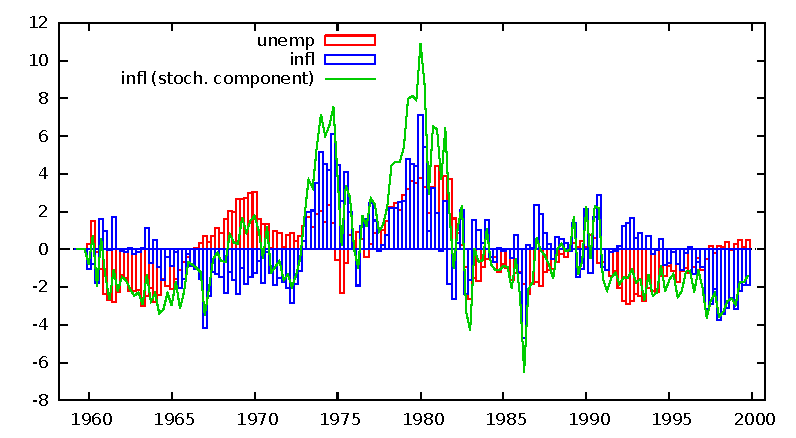
\includegraphics[scale=0.8]{Cmodel_hd}
  \caption{Simple C-model example: historical decomposition plot}
  \label{fig:Cmodel-hd}
\end{figure}

A traditional way to represent the outcome of historical decomposition
is, again, graphical. The most common variant depicts the single
contributions as histograms against time and their sum (the stochastic
component $y_t - d_t$) as a continuous line. The SVAR package provides
a pair of functions for plotting such a graph on screen or saving it
to a file, and the go by the name of \cmd{HDplot()} and
\cmd{HDsave()}, respectively. See their description in Section
\ref{sec:syntax} in the appendix and Figure \ref{fig:Cmodel-hd}, which
shows the historical decomposition for the unemployment series we've
been using as an example in this section.

\section{C-models with long-run restrictions (Blanchard-Quah style)}
\label{sec:BlQuah}

\begin{table}[htbp]
\begin{scode}
set echo off
set messages off
include SVAR.gfn
open BlQuah.gdt

list X = DY U
list exog = const time
maxlag = 8

# set up the model
BQModel = SVAR_setup("C", X, exog, maxlag)
BQModel.horizon = 40

# set up the long-run restriction
SVAR_restrict(&BQModel, "lrC", 1, 2, 0)

# cumulate the IRFs for variable 1
SVAR_cumulate(&BQModel, 1)

# set up names for the shocks
BQModel.snames = strsplit("Supply Demand")

# do estimation
SVAR_estimate(&BQModel)

# retrieve the demand shocks
dShock = GetShock(&BQModel, 2)

# bootstrap
bfail = SVAR_boot(&BQModel, 1024, 0.9)

# page 662
IRFsave("bq_Yd.pdf", &BQModel,  1, 1)
IRFsave("bq_ud.pdf", &BQModel, -2, 1)
IRFsave("bq_Ys.pdf", &BQModel,  1, 2)
IRFsave("bq_us.pdf", &BQModel, -2, 2)

# now perform historical decomposition
list HDDY = SVAR_hd(&BQModel, 1)
list HDU  = SVAR_hd(&BQModel, 2)

# cumulate the effect of the demand shock on DY
series hd_Y_Demand = cum(hd_DY_Demand)
# reproduce Figure 8
gnuplot hd_Y_Demand --time-series --with-lines --output=display

# reproduce Figure 10
gnuplot hd_U_Demand --time-series --with-lines --output=display    

\end{scode}
  \caption{Blanchard-Quah example}
  \label{tab:BlQuah}
\end{table}

An alternative way to impose restrictions on $C$ is to use long-run
restrictions, as pioneered by \cite{BlanQuah1}. The economic
rationale of imposing restrictions on the elements of $C$ is that $C$
is equal to $M_0$, the instantaneous IRF. For example, Cholesky-style
restrictions mean that the $j$-th shock has no instantaneous impact on
the $i$-th variable if $i<j$. Assumptions of this kind are normally
motivated by institutional factors such as sluggish adjustments,
information asymmetries, technical constraints and so on.

Long-run restrictions, instead, stem from more theoretically-inclined
reasoning: in \cite{BlanQuah1}, for example, it is argued that in the
long run the level of GDP is ultimately determined by aggregate supply
only. Fluctuations in aggregate demand, such as those induced by
fiscal or monetary policy, should affect the level of GDP only in the
short term. As a consequence, the impulse response of GDP with respect
to demand shocks should go to 0 asymptotically, whereas the response
of GDP to a supply shock should settle to some positive value.

\subsection{A modicum of theory}
To translate this intuition into formulae, assume that the bivariate
process GDP growth-unemployment
\[
  x_t = \left[ \begin{array}{c} \Delta Y_t \\ U_t  \end{array}\right]
\]
is $I(0)$ (which implies that $Y_t$ is $I(1)$), and that it admits a
finite-order VAR representation
\[
  \VarSym(L) x_t = \PrE{t} 
\]
where the prediction errors are assumed to be a linear combination of
demand and supply shocks
\[
  \left[ \begin{array}{c} \PrE{t}^{\Delta Y} \\ \PrE{t}^U  \end{array}\right] 
  = 
  C \left[ \begin{array}{c} \StS{t}^d \\ \StS{t}^s  \end{array}\right] ,
\]

Considering the structural VMA representation
\begin{eqnarray*}
  \left[ \begin{array}{c} \Delta Y_t \\ U_t \end{array}\right] & = & 
  \Theta(L) \PrE{t} =
  \PrE{t} + \Theta_1 \PrE{t-1}  + \cdots = \\
  & = & C \StS{t} + \Theta_1 C \StS{t-1}  + \cdots =
  M_0 \StS{t} + M_1 \StS{t-1}  + \cdots ,
\end{eqnarray*}
it should be clear that the impact of demand shocks on $\Delta Y_t$
after $h$ periods is given by the north-west element of $M_h$. Since
$x_t$ is assumed to be stationary, $\lim_{h \to \infty} \Theta_h = 0$
and the same holds for $M_k$, so obviously the impact of either shock
on $\Delta Y_t$ goes to 0. However, the impact of $u_t$ on the
\emph{level} of $Y_t$ is given by the \emph{sum} of the corresponding
elements of $M_h$, since
\[
Y_{t+h} = Y_{t-1} + \sum_{i=0}^h \Delta Y_{t+i}, 
\]
so 
\[
  \pder{Y_{t+h}}{\StS{t}^d} = 
  \sum_{i=0}^h \pder{\Delta Y_{t+i}}{\StS{t}^d} = 
  \sum_{i=0}^h \left[M_i\right]_{11}
\]
and in the limit
\[
\lim_{h \to \infty} \pder{Y_{t+h}}{\StS{t}^d} = \sum_{i=0}^{\infty}
\pder{\Delta Y_{t+i}}{\StS{t}^d}  = 
  \sum_{i=0}^{\infty} \left[M_i\right]_{11},
\]

In general, if $x_t$ is stationary, the above limit is finite, but
needn't go to 0; however, if we assume that the long-run impact of
$\StS{t}^d$ on $Y_t$ is null, then
\[
  \lim_{k \to \infty} \pder{Y_{t+k}}{\StS{t}^d} = 0
\]
and this is the restriction we want. In practice, instead of
constraining elements of $M_0$, we impose an implicit constraint on
the whole sequence $M_i$.

How do we impose such a constraint?  First, write $\sum_{i=0}^{\infty}
\Theta_i$ as $\Theta(1)$; then, observe that
\[
  \Theta(1) C = \sum_{i=0}^{\infty} M_i ;
\]
the constraint we seek is that the north-west element of $\Theta(1) C$
equals 0. The matrix $\Theta(1)$ is easy to compute after the VAR
coefficients have been estimated: since $\Theta(L) = \VarSym(L)^{-1}$, an
estimate of $\Theta(1)$ is simply
\[
  \widehat{\Theta(1)} = \widehat{\VarSym(1)}^{-1}
\]
Of course, for this to work $\VarSym(1)$ needs to be invertible. This rules
out processes with one or more unit roots. The cointegrated case,
however, is an interesting related case and will be analysed in section
\ref{sec:SVECs}.

The long-run constraint can then be written as
\begin{equation}
  \label{eq:BQlongrun}
  R \VEC[\Theta(1) C] = 0, 
\end{equation}
where $R = \left[ 1, 0, 0, 0 \right]$; since 
\[
  \VEC[\Theta(1) C] = [I \otimes \Theta(1)] \VEC(C), 
\]
the constraint can be equivalently expressed as
\begin{equation}
  \label{BQlongrun2}
  \left[ \Theta(1)_{11}, \Theta(1)_{12}, 0, 0 \right] \VEC(C) = 
  \Theta(1)_{11} \cdot c_{11} + \Theta(1)_{12} \cdot c_{21} = 0.
\end{equation}
Note that we include in $R$ elements that, strictly speaking, are not
constant, but rather functions of the estimated VAR parameters. Bizarre
as this may seem, this poses no major inferential problems under a
suitable set of conditions (see \cite{AG}, section 6.1).

\begin{table}[htbp]
\begin{scode}
             coefficient   std. error      z       p-value 
  ---------------------------------------------------------
  C[ 1; 1]    0.0575357    0.0717934      0.8014   0.4229  
  C[ 2; 1]    0.217542     0.0199133     10.92     8.80e-28 ***
  C[ 1; 2]   -0.907210     0.0507146    -17.89     1.45e-71 ***
  C[ 2; 2]    0.199459     0.0111501     17.89     1.45e-71 ***

Bootstrap results (1000 replications)

             coefficient   std. error      z      p-value 
  --------------------------------------------------------
  C[ 1; 1]     0.232452    0.285316      0.8147   0.4152  
  C[ 2; 1]     0.191064    0.0786388     2.430    0.0151   **
  C[ 1; 2]    -0.829021    0.113861     -7.281    3.31e-13 ***
  C[ 2; 2]     0.222009    0.0648956     3.421    0.0006   ***
\end{scode}
  \caption{Output for the Blanchard-Quah model}
  \label{tab:BlQuahOutput}
\end{table}

\subsection{Example}
The way all this is handled in \texttt{SVAR} is hopefully quite
intuitive: an example script is reported in Table
\ref{tab:BlQuah}. After reading the data in, the function
\texttt{SVAR\_setup} is invoked in pretty much the same way as in
section \ref{sec:Cmodel}.

Then, the \texttt{SVAR\_restrict} is used to specify the identifying
restriction. Note that in this case the code for the restriction type
is \texttt{"lrC"}, which indicates that the restriction applies to the
long-run matrix, so the formula \eqref{BQlongrun2} is employed. Next,
we insert into the model the information that we will want IRFs for
$y_t$, so those for $\Delta y_t$ will have to be cumulated. This is
done via the function \texttt{SVAR\_cumulate()}, in what should be a
rather self-explanatory way (the number 1 refers in this case to the
position of $\Delta Y_t$ in the list \texttt{X}). Finally, a cosmetic
touch: we store into the model the string array \texttt{"Supply"} and
\texttt{"Demand"}, which will be used to label the shocks in the
graphs. Note that in this case there is no ad-hoc function, but we
rely on the standard \app{gretl} syntax for bundles.

\begin{figure}[htbp]
 \centering
  %\hspace{-1cm}
  \begin{tabular}{cc}
    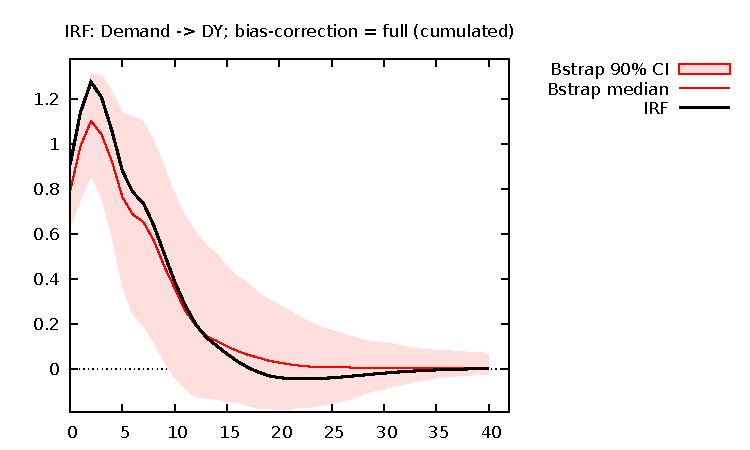
\includegraphics[width=\irfw, height=\irfh]{bq_Yd} &
    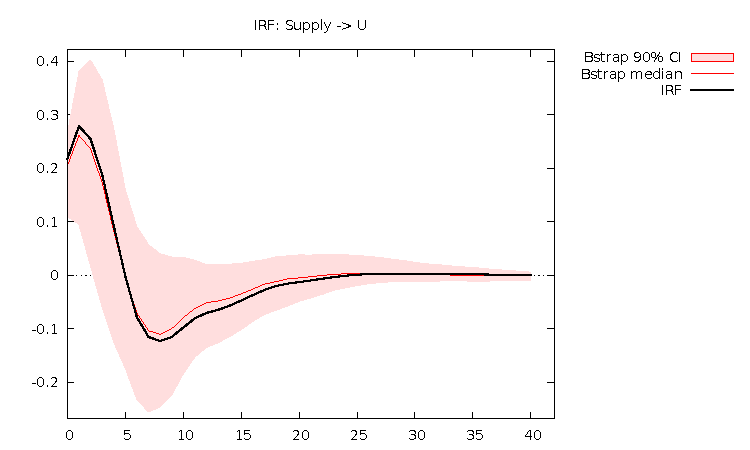
\includegraphics[width=\irfw, height=\irfh]{bq_Ys} \\
    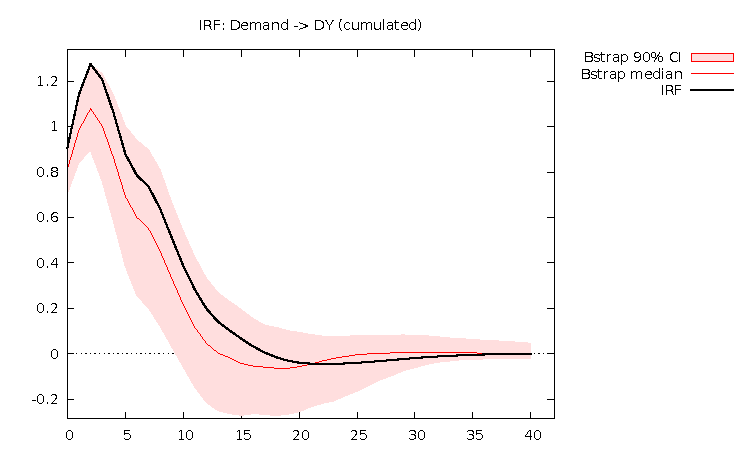
\includegraphics[width=\irfw, height=\irfh]{bq_ud} &
    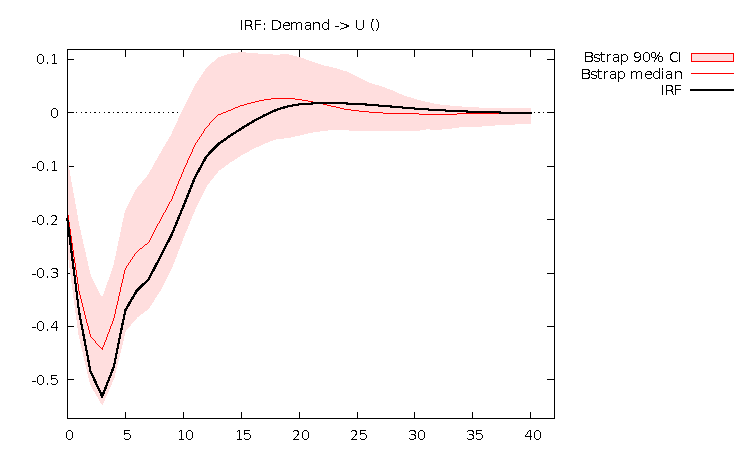
\includegraphics[width=\irfw, height=\irfh]{bq_us}
  \end{tabular}
  \caption{Impulse response functions for the Blanchard-Quah model}
  \label{fig:BlQuah}
\end{figure}

In Table \ref{tab:BlQuahOutput} I reported the output to the example
code in Table \ref{tab:BlQuah}, while the pretty pictures are in
Figure \ref{fig:BlQuah}.\footnote{I found it impossible to reproduce
  Blanchard and Quah's results \emph{exactly}. I believe this is due
  to different vintages of the data. Qualitatively, however, results
  are very much the same. } Note that in the two calls to
\texttt{IRFplot} which are used to plot the responses to a demand
shock, the number to identify the shock is not 2, but rather -2. This
is a little trick the plotting functions use to flip the sign of the
impulse responses, which may be necessary to ease their interpretation
(since the shocks are identified only up to their sign).

Note that the bottom part of the scripts uses the functions described
in section \ref{sec:HD} so to replicate figures 8 (p.~664) and 10
(p.~665) in the original AER article, where the historical
contribution of demand shocks to output and unemployment is
reconstructed. The output on your screen should be roughly similar to
figure \ref{fig:BlQuah-HD-Output}.

\begin{figure}[hbtp]
  \centering
  \begin{tabular}{cc}
    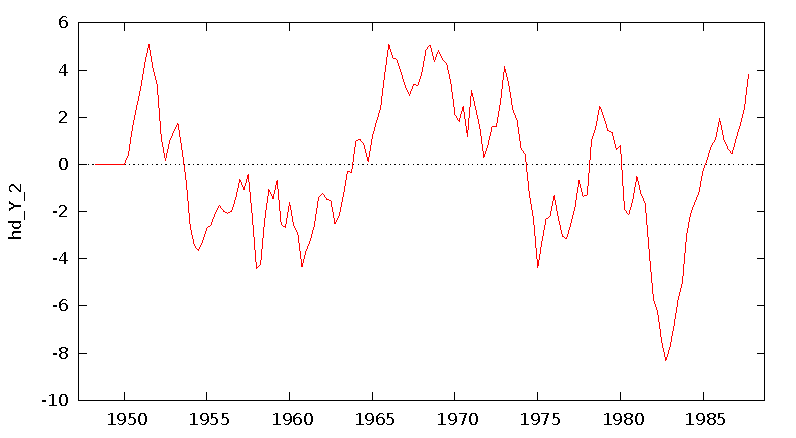
\includegraphics[width=0.45\textwidth]{bqhdy} &
    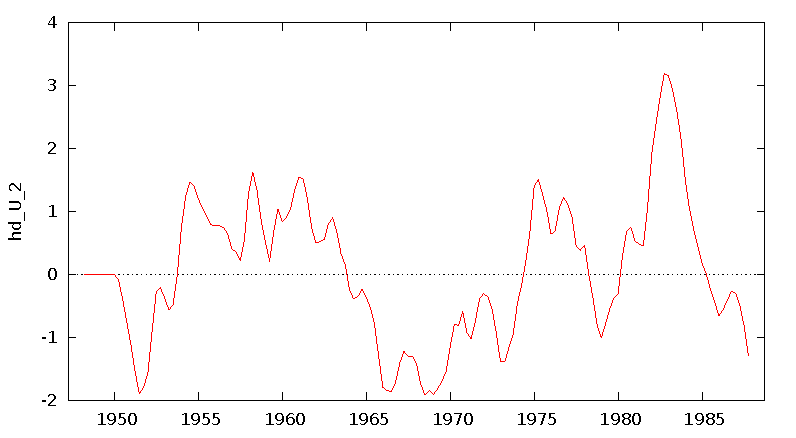
\includegraphics[width=0.45\textwidth]{bqhdu} \\
    Output & Unemployment
  \end{tabular}
  \caption{Effects of a demand shock in the Blanchard-Quah model}
  \label{fig:BlQuah-HD-Output}
\end{figure}

\subsection{Combining short- and long-run restrictions}
\label{sec:C-combined}

In the previous example, it turned out that the estimated coefficient
for $c_{1,1}$ was seemingly insignificant; if true, this would mean
that the supply shock has no instantaneous effect on $\Delta Y_t$; in
other words, the IRF of output to supply starts from 0. Leaving the
economic implications aside, from a statistical viewpoint this could
have suggested an alternative identification strategy or, more
interestingly, to combine the two hypotheses into one. 

The script presented in Table \ref{tab:BlQuah} is very easy to modify
to this effect: in this case, we simply need to insert the line 
\begin{code}
  SVAR_restrict(&BQModel, "C", 1, 1, 0)
\end{code}
somewhere between the \texttt{SVAR\_setup} and the
\texttt{SVAR\_estimate} function. 
The rest is unchanged, and below is the output.

\begin{code}
             coefficient   std. error     z       p-value 
  --------------------------------------------------------
  C[ 1; 1]     0.00000     0.00000       NA      NA       
  C[ 2; 1]    -0.230192    0.0128681    -17.89    1.45e-71 ***
  C[ 1; 2]    -0.909033    0.0508165    -17.89    1.45e-71 ***
  C[ 2; 2]     0.199859    0.0111725     17.89    1.45e-71 ***

Overidentification LR test = 0.642254 (1 df, pval = 0.422896)
\end{code}

Note that, since this model is over-identified, \texttt{SVAR}
automatically computes a LR test of the overidentifying
restrictions. Of course, all the subsequent steps (bootstrapping and
IRF plotting) can be performed just like in the previous example if
so desired.

\section{AB models}
\label{sec:ABmodels}
\subsection{A simple example}

\begin{table}[htbp]
  \begin{scode}
set echo off
set messages off
include SVAR.gfn
open IS-LM.gdt

list X = q i m
list Z = const time

ISLM = SVAR_setup("AB", X, Z, 4)
ISLM.horizon = 48

SVAR_restrict(&ISLM, "Adiag", 1)
SVAR_restrict(&ISLM, "A", 1, 3, 0)
SVAR_restrict(&ISLM, "A", 3, 1, 0)
SVAR_restrict(&ISLM, "A", 3, 2, 0)
SVAR_restrict(&ISLM, "Bdiag", NA)
ISLM.snames = "uIS uLM uMS"
SVAR_estimate(&ISLM)

Amat = ISLM.S1
Bmat = ISLM.S2

printf "Estimated contemporaneous impact matrix (x100) =\n%10.6f", \
  100*inv(Amat)*Bmat

rej = SVAR_boot(&ISLM, 2000, 0.95)
IRFplot(&ISLM, 1, 2)
  \end{scode}
  \caption{Estimation of an AB model --- example from \cite{LKBook04}}
  \label{tab:ABmodel}
\end{table}
AB models are more general than the C model, but more rarely used in
practice. In order to exemplify the way in which they are handled in
the \texttt{SVAR} package, I will replicate the example given in
section 4.7.1 of  \cite{LKBook04}. See Table
\ref{tab:ABmodel}.

This is an empirical implementation of a standard Keynesian IS-LM
model in the formulation by \cite{Pagan95}. The vector of endogenous
variables includes output $q_t$, interest rate $i_t$ and real money
$m_t$; the matrices $A$ and $B$ are
\[
A = \left[ \begin{array}{ccc}
    1 & a_{12} & 0 \\ a_{21} & 1 & a_{31} \\ 0 & 0 & 1
  \end{array} \right]
\qquad
B = \left[ \begin{array}{ccc}
    b_{11} & 0 & 0 \\ 0 & b_{22} & 0 \\ 0 & 0 & b_{33}
  \end{array} \right]
\]
so for example the first structural relationship is
\begin{equation}
  \label{eq:AB-IScurve}
  \PrE{t}^q = -a_{12} \PrE{t}^i + \StS{t}^{IS}
\end{equation}
which can be read as an IS curve. The LM curve is the second
relationship, while money supply is exogenous.

The model is set up via the function \texttt{SVAR\_setup}, like in the
previous section. Note, however, that in this case the model code is
\texttt{"AB"} rather than \texttt{"C"}.  The base VAR has 4 lags, with
the constant and a linear time trend as exogenous variables. The
horizon of impulse response analysis is set to 48 quarters.

The constraints on the matrices $A$ and $B$ can be set up quite simply
by using a the function \texttt{SVAR\_restrict} via a special syntax
construct: the line
\begin{code}
  SVAR_restrict(&ISLM, "Adiag", 1)
\end{code}
sets up a system of constraints such that all elements on the diagonal
of $A$ are set to 1. More precisely, \texttt{SVAR\_restrict(\&Model,
  "Adiag", x)} sets all diagonal elements of $A$ to the value $x$,
unless $x$ is \texttt{NA}. In that case, all \emph{non-diagonal}
elements are constrained to 0, while diagonal elements are left
unrestricted; in other words, the syntax
\begin{code}
  SVAR_restrict(&ISLM, "Bdiag", NA)
\end{code}
is a compact form for saying ``$B$ is diagonal''. The other three
constraints are set up as usual.

Estimation is then carried out via the \texttt{SVAR\_estimate}
function; as an example, Figure \ref{fig:Dynamic-IS} shows the effect
on the interest rate of a shock on the IS curve.  This example also
shows how to retrieve estimated quantities from the model: after
estimation, the bundle elements \texttt{S1} and \texttt{S2}
contain the estimated $A$ and $B$ matrices; the $C$ matrix is then
computed and printed out.

The output is shown below:

\begin{code}
             coefficient   std. error      z       p-value 
  ---------------------------------------------------------
  A[ 1; 1]    1.00000       0.00000     NA        NA       
  A[ 2; 1]   -0.144198      0.280103    -0.5148    0.6067  
  A[ 3; 1]    0.00000       0.00000     NA        NA       
  A[ 1; 2]   -0.0397571     0.155114    -0.2563    0.7977  
  A[ 2; 2]    1.00000       0.00000     NA        NA       
  A[ 3; 2]    0.00000       0.00000     NA        NA       
  A[ 1; 3]    0.00000       0.00000     NA        NA       
  A[ 2; 3]    0.732161      0.146135     5.010     5.44e-07 ***
  A[ 3; 3]    1.00000       0.00000     NA        NA       


             coefficient   std. error      z      p-value 
  --------------------------------------------------------
  B[ 1; 1]   0.00671793    0.000473619   14.18    1.15e-45 ***
  B[ 2; 1]   0.00000       0.00000       NA      NA       
  B[ 3; 1]   0.00000       0.00000       NA      NA       
  B[ 1; 2]   0.00000       0.00000       NA      NA       
  B[ 2; 2]   0.00858125    0.000581359   14.76    2.63e-49 ***
  B[ 3; 2]   0.00000       0.00000       NA      NA       
  B[ 1; 3]   0.00000       0.00000       NA      NA       
  B[ 2; 3]   0.00000       0.00000       NA      NA       
  B[ 3; 3]   0.00555741    0.000371320   14.97    1.21e-50 ***

Estimated contemporaneous impact matrix (x100) =
  0.675666  0.034313 -0.016270
  0.097430  0.863073 -0.409238
  0.000000  0.000000  0.555741

Bootstrap results (2000 replications)

             coefficient   std. error      z       p-value 
  ---------------------------------------------------------
  A[ 1; 1]    1.00000       0.00000     NA        NA       
  A[ 2; 1]   -0.0909784     0.395312    -0.2301    0.8180  
  A[ 3; 1]    0.00000       0.00000     NA        NA       
  A[ 1; 2]   -0.0377229     0.228185    -0.1653    0.8687  
  A[ 2; 2]    1.00000       0.00000     NA        NA       
  A[ 3; 2]    0.00000       0.00000     NA        NA       
  A[ 1; 3]    0.00000       0.00000     NA        NA       
  A[ 2; 3]    0.782728      0.181538     4.312     1.62e-05 ***
  A[ 3; 3]    1.00000       0.00000     NA        NA       


             coefficient   std. error      z       p-value 
  ---------------------------------------------------------
  B[ 1; 1]   0.00635862    0.000850539    7.476    7.66e-14 ***
  B[ 2; 1]   0.00000       0.00000       NA       NA       
  B[ 3; 1]   0.00000       0.00000       NA       NA       
  B[ 1; 2]   0.00000       0.00000       NA       NA       
  B[ 2; 2]   0.00814276    0.00111305     7.316    2.56e-13 ***
  B[ 3; 2]   0.00000       0.00000       NA       NA       
  B[ 1; 3]   0.00000       0.00000       NA       NA       
  B[ 2; 3]   0.00000       0.00000       NA       NA       
  B[ 3; 3]   0.00512819    0.000478826   10.71     9.14e-27 ***
\end{code}

\begin{figure}[htbp]
  \centering
  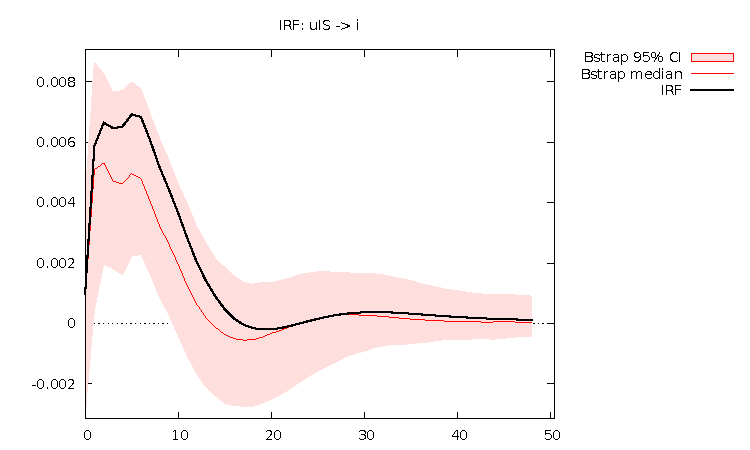
\includegraphics{dynamic_IS}
  \caption{$\StS{}^{IS} \to i$}
  \label{fig:Dynamic-IS}
\end{figure}

\section{Checking for identification}
\label{sec:SVARid}

Consider equation \eqref{eq:PrE-StS-AB} again, which we reproduce
here for clarity:
\[
  A \PrE{t} = B \StS{t}
\]
Since the $\StS{t}$ are assumed mutually incorrelated with unit variance,
the following relation must hold:
\begin{equation}
  \label{eq:AB-Sigma}
  A \Sigma A' = B B'
\end{equation}
If $C \equiv A^{-1}B$, equation (\ref{eq:AB-Sigma}) can be written as
\[
  \Sigma = C C'.
\]

The matrix $\Sigma$ can be consistently estimated via the sample
covariance matrix of VAR residuals, but estimation of $A$ and $B$ is
impossible unless some constraints are imposed on both matrices:
$\hat{\Sigma}$ contains $\frac{n (n+1)}{2}$ distinct entries; clearly,
the attempt to estimate $2 n^2$ parameters violates an elementary
order condition. 

The recursive identification scheme resolves the issue by fixing $A=I$
and by imposing lower-triangularity of $B$. In general, however, one
may wish to achieve identification by other means.\footnote{Necessary
  and sufficient conditions to achieve identification are stated in
  \cite{ET06}. Other interesting contributions in this area is
  \cite{RR-W-Zha10} and \cite{Bacchiocchi11}.}  The most immediate way
to place enough constraints on the $A$ and $B$ matrices so to achieve
identification is to specify a system of linear constraints; in other
words, the restrictions on $A$ and $B$ take the form
\begin{eqnarray}
  \label{eq:ImpConstA}
  R_a \VEC A & = & d_a \\
  \label{eq:ImpConstB}
  R_b \VEC B & = & d_b 
\end{eqnarray}
% So in practice the only potentially meaningful cases that are ruled
% out are nonlinear restrictions and cross-matrix restrictions.

This setup is perhaps overly general in most cases: the restrictions
that are put almost universally on $A$ and $B$ are zero- or
one-restrictions, that is constraints of the form, eg, $A_{ij} = 1$. In
these cases, the corresponding row of $R$ is a vector with a 1 in a
certain spot and zeros everywhere else. However, generality is nice
for exploring the identification problem.

The order condition demands that the number of restrictions is at
least $2 n^2 - \frac{n (n+1)}{2} = n^2 + \frac{n (n-1)}{2}$, so for
the order condition to be fulfilled it is necessary that
\begin{eqnarray*}
  0 < & \rk{R_a} & \le n^2 \\
  0 < & \rk{R_b} & \le n^2 \\
  n^2 + \frac{n (n-1)}{2} \le & \rk{R_a} + \rk{R_b} & \le 2 n^2
\end{eqnarray*}

For the C model, $R_a = I_{n^2}$ and $d_a = \VEC I_n$, so to satisfy
the order condition $\frac{n (n-1)}{2}$ constraints are needed on on
$B$: in practice, for a C model we have one set of constraints which
pertain to $B$, or, equivalently in this context, to $C$:
\begin{equation}
  \label{eq:ImpConstC}
  R \VEC C = d
\end{equation}

The problem is that the order condition is necessary, but not
sufficient. It is possible to construct models in which the order
condition is satisfied but there is an uncountable infinity of
solutions to the equation $A \Sigma A' = B B'$. If you try to estimate
such a model, you're bound to hit all sorts of numerical problems
(apart from the fact, of course, that your model will have no
meaningful economic interpretation).

In order to ensure identification, another condition, called the
\emph{rank} condition, has to hold together with the order
condition. The rank condition is described in \cite{AG} (chapter 4 for
the AB model), and it involves the rank of a certain matrix, which can
be computed as a function of the four matrices $R_a$, $d_a$, $R_b$ and
$d_b$. The \texttt{SVAR} package contains a function for doing just
that, whose name is \texttt{SVAR\_ident}.

As a simple example, let's check that the plain model is in fact
identified by running a simple variation of the example contained in
Table \ref{tab:simpleC-base}: 

\begin{code}
set echo off
set messages off

include SVAR.gfn
open sw_ch14.gdt

genr infl = 400*ldiff(PUNEW)
rename LHUR unemp

list X = unemp infl
list Z = const

Mod = SVAR_setup("C", X, Z, 3)
SVAR_restrict(&Mod, "C", 1, 2)

# Now check for identification
scalar is_identified = SVAR_ident(&Mod)
if is_identified
    printf "Whew!\n"
else
    printf "Blast!\n"
endif

# Re-check, verbosely
scalar is_identified = SVAR_ident(&Mod, 1)
\end{code}

The above code should produce the following output:

\begin{code}
Order condition OK
Rank condition OK
Whew!
Constraints in implicit form:

Ra:
   1   0   0   0
   0   1   0   0
   0   0   1   0
   0   0   0   1

da:
   1
   0
   0
   1

Rb:
   0   0   1   0

db:
   0

no. of constraints on A: 4
no. of constraints on B: 1
no. of total constraints: 5
no. of necessary restrictions for the order condition = 5
Order condition OK
rank condition: r = 5, cols(Q) = 5
Rank condition OK
\end{code}
\section{Structural VEC Models}
\label{sec:SVECs}

This class of models was first proposed in \cite{KPSW91}.\footnote{A
  very nice paper in the same vein which is also frequently cited is
  \cite{GoNg2001}. A compact yet rather complete analysis of the main
  issues in this context can be found in \cite{Lut06}.} A SVEC is
basically a C-model in which the interest is centred on classifying
structural shocks as permanent or transitory by exploiting the
presence of cointegration.

Suppose we have an $n$-dimensional system with cointegration rank $r$
which can be represented as a finite-order VAR $\VarSym(L) y_t =
\PrE{t}$. As is well known,\footnote{See \cite{joha-book}.} the system
also admits the VECM representation
\begin{equation}
  \label{eq:VECM}
  \Gamma(L) \Delta y_t = \mu_t + \alpha \beta' y_{t-1} + \PrE{t}
\end{equation}
in which $\alpha$ and $\beta$ are $r \times n$ matrices, with $0 \le r
\le n$. If $r=n$, the system is stationary; if $r=0$, the system is
$I(1)$. In the intermediate cases, $r$ is said to be the
\emph{cointegration rank}.

In all these cases, it is also possible to express $\Delta y_{t}$ as a
vector moving average process
\begin{equation}
  \label{eq:coint-VMA}
  \Delta y_t = C(L) \PrE{t} .
\end{equation}
The main consequence of cointegration for eq.~(\ref{eq:coint-VMA}) is
that $C(1)$ is a singular matrix, with rank $n-r$.  The most important
consequence of the above for structural estimation is that the $C(1)$
matrix satisfies
\[
  C(1) \alpha = 0 ;
\]
Moreover, as argued in section \ref{sec:BlQuah}, the $ij$-th element
of $C(1)$ can be thought of as the long-run response of $y_{i,t}$ to
$\PrE{j,t}$ or, more precisely
\[
  C(1)_{ij} = \lim_{k \to \infty} \pder{y_{i, t+k}}{\PrE{j, t}}.
\]
Hence, the long-run response of $y_t$ to structural shocks is easily
seen (via eq.~\ref{eq:PrE-StS-C}) to be $C(1) \cdot C$.

Now, define a transitory shock as a structural shock that has no
long-run effect on any variable: therefore, the corresponding column
of $C(1) \cdot C$ must be full of zeros. But this, in turn, implies
that the corresponding column of $C$ must be a linear combination of
the columns of $\alpha$. Since $\alpha$ has $r$ linearly independent
columns, the vector of structural shocks must contain $r$ transitory
shocks and $n-r$ permanent ones.

By ordering the structural shocks with the permanent ones first,
\[
  \StS{t} = \left[ \begin{array}{c} \StS{t}^p \\ \StS{t}^t  \end{array}\right] 
\] 
it's easy to see that a separation of the transitory shocks from the
permanent ones can be achieved by imposing that the last $r$ columns
of $C$ lie in the space spanned by $\alpha$; in formulae,
\begin{equation}
  \label{eq:SVEC-id}
  \alpha_{\perp}' C J = 0 ,
\end{equation}
where $J$ is the matrix 
\[ 
  J = \left[ \begin{array}{c} 0_{n-r \times r} \\ 
      I_{r\times r}  \end{array}\right] 
\]
and $\perp$ is the ``nullspace'' operator.\footnote{If $M$ is an $r
  \times c$ matrix, with $r>c$ and $\rk{M} = c$, then $M_{\perp}$ is
  some matrix such that $M_{\perp}'M = 0$.  Note that $M_{\perp}$ is
  not unique.} Equation \eqref{eq:SVEC-id} can be expressed in vector
form as
\[
  ( J' \otimes \alpha_{\perp}' ) \VEC(C)  = 0 ;
\]
since $\alpha_{\perp}$ has $n-r$ columns, this provides $r\cdot(n-r)$
constraints of the type $R \VEC(C) = d$, that we know how to handle.

Since $0 < r < n$, this system of constraints is not sufficient to
achieve identification, apart from the special case $n =2$, $r=1$, so
in general the partition between transitory and permanent shocks must
be supplemented by extra constraints. Clearly, these can be short-run
constraints on both kind of shocks, but long-run constraints only make
sense on permanent ones.

\subsection{Syntax}
\label{sec:KPSWsyntax}

Fort this type of model, the model code you have to supply to
\cmd{SVAR\_setup} is \cmd{"SVEC"}. This means that your model is a
C-model in which, however, the structural shocks will be classified as
transitory or permanent, depending on the cointegration properties you
assume.

This is an important point: \texttt{SVAR} is not meant for doing
inference on the cointegration part of your model. For determining the
cointegration rank of your system and estimating the cointegration
$\beta$, you're on your own. Of course, you can use \app{gretl}'s
in-built commands, such as \cmd{coint2} and \cmd{vecm}, or pre-set
them to some theory-derived value: \texttt{SVAR} won't care, and will
blindly accept the matrix $\beta$ you supply it; the cointegration
rank is implicitly assumed as the number of columns of the $\beta$
matrix.

Another piece of information you must supply separately, prior to
estimation, is how you want the deterministic terms (the constant and
the trend) in your model to be treated; in practice, which of the
famous ``five cases'' you want to apply to your model. In fact, the
constant and the trend are subject to a special treatment in this
class of models, so they will be dropped from the exogenous list
\texttt{X}, if present, when you call \cmd{SVAR\_setup} and re-added
internally if needed. Unless you have extra exogenous variables, such
as centred seasonals, you might just as well leave \texttt{X} as
\texttt{null}. The five cases range from the most to the least
restrictive, as per Table \ref{tab:5cases}.

\begin{table}[htbp]
  \centering
  \begin{tabular}{rrl}
    \hline
    Code & \cmd{vecm} option & Description\\
    \hline
    1 & \option{nc} & No constant, no trend \\
    2 & \option{rc} & Restricted constant, no trend \\
    3 &  & Unrestricted constant, no trend \\
    4 & \option{crt} & Constant, restricted trend \\
    5 & \option{ct} & Constant, unrestricted trend \\
    \hline
  \end{tabular}
  \caption{The five cases for deterministic terms in cointegrated systems}
  \label{tab:5cases}
\end{table}

This is not the place for explaining the differences between the five
options; if you've come this far, you probably know already. If you
don't, grab any decent econometrics textbook or the \emph{Gretl User's
  Guide} and look for the chapter on cointegration and VECMs.

For injecting the necessary information into the model bundle once
you've set it up, there is a dedicated function whose name is
\texttt{SVAR\_coint}. It takes four compulsory parameters: the SVAR
model (in pointer form), the ``deterministic terms code'' and the
matrices $\beta$ and $\alpha$; the latter may be empty, in which case
it will be estimated via OLS. If, on the contrary, it is not empty,
then it should be a $n \times r$ matrix that will be accepted at face
value. Pre-setting $\alpha$ may be useful, in some cases, to force
some of the variables to be weakly exogenous. Note that the
\verb!$jbeta!  and \verb|$jalpha| standard gretl accessors make it
painless to fetch them from a Johansen-style VECM if necessary.

Calling this function will
\begin{enumerate}
\item set up a system of constraints such that the $n-r$ permanent
  shocks will come first in the ordering, followed by the $r$
  temporary ones. The shock names will be set accordingly.
\item Estimate the VECM parameters subject to the constraints implied
  by the given $\beta$ (and $\alpha$, if not empty): in practice, the
  matrix $\Sigma$ and the parameters $\mu$ and $\Gamma_i$ in equation
  \eqref{eq:VECM}. Internally, \texttt{SVAR\_coint} will take care of
  transforming into the VAR form \eqref{eq:VAR} so that the VMA
  representation can be computed and everything will proceed like in
  an ordinary C model.
\end{enumerate}

At that point, the rest of the model can be setup as per usual
(setting extra restrictions and so on). In the next subsection, I will
provide an extended and annotated example.


\begin{table}[htbp]
  \begin{scode}
     1	nulldata 116
     2	setobs 4 1970:1 
     3	include SVAR.gfn
     4	
     5	# grab data from AWM 
     6	join AWM.gdt YER PCR ITR
     7	
     8	# transform into logs
     9	series y = 100 * ln(YER)
    10	series c = 100 * ln(PCR)
    11	series i = 100 * ln(ITR)
    12	list X = c i y
    13	
    14	# find best lag
    15	var 8 X --lagselect
    16	p = 3
    17	
    18	# check for the "balanced growth path" hypothesis
    19	coint2 p X 
    20	vecm p 2 X
    21	restrict
    22	    b[1,1] = -1
    23	    b[1,2] =  0
    24	    b[1,3] =  1
    25	    
    26	    b[2,1] =  0
    27	    b[2,2] = -1
    28	    b[2,3] =  1
    29	end restrict
    30	
    31	# ok, now go for the real thing
    32	x = SVAR_setup("SVEC", X, const, p)
    33	matrix b = I(2) | -ones(1,2)
    34	SVAR_coint(&x, 3, b, {}, 1)
    35	x.horizon = 40		 
    36	SVAR_restrict(&x, "C", 1, 2, 0)	 
    37					 
    38	SVAR_estimate(&x)		 
    39	loop j=1..3 --quiet		 
    40	    FEVDplot(&x, j)		 
    41	endloop				 
    42					 
    43	SVAR_boot(&x, 1024, 0.90) 
    44	loop j=1..3 --quiet				 
    45	    IRFplot(&x, 1, j, 2)
    46	endloop		     		 
  \end{scode}
  \caption{The \texttt{awm.inp} script}
    \label{tab:awmscript}
\end{table}

\subsection{A hands-on example}
\label{sec:KPSWexample}

In this example, we will go through a pseudo-replication of the
simpler of the two examples presented in \cite{KPSW91}: the structure
of the model will be kept the same, but we will use a different
dataset. While the original article used post-WWII data for the US
economy, I will use the so-called AWM dataset, which is supplied among
\app{gretl}'s sample datasets. AWM stands for Area-Wide Model, and is
a quarterly dataset of the Euro area, which spans the 1970-1998
period. It was originally developed by \cite{AWM} but has been used in
countless other benchmark studies. The script is supplied in the
examples directory as \texttt{awm.inp}, but we reproduce it here as
table \ref{tab:awmscript} for your convenience.

The model comprises three variables, all in logs: real GDP ($y_t$),
real private consumption ($c_t$) and real investment ($i_t$); these
should, in theory, follow the same stochastic trend (the so-called
``balanced growth path''), so that there ought to be two cointegration
relationships:
\begin{eqnarray*}
  c_t &=& y_t + z^c_t \\
  i_t &=& y_t + z^i_t
\end{eqnarray*}

The general idea of the script is: use \app{gretl}'s internal
functions to estimate the VECM and test whether the ``balanced growth
path'' hypothesis is in fact tenable on this particular dataset. Then,
set up the structural part of the model, estimate it and do a few
plots.

\begin{figure}[htbp]
  \centering
  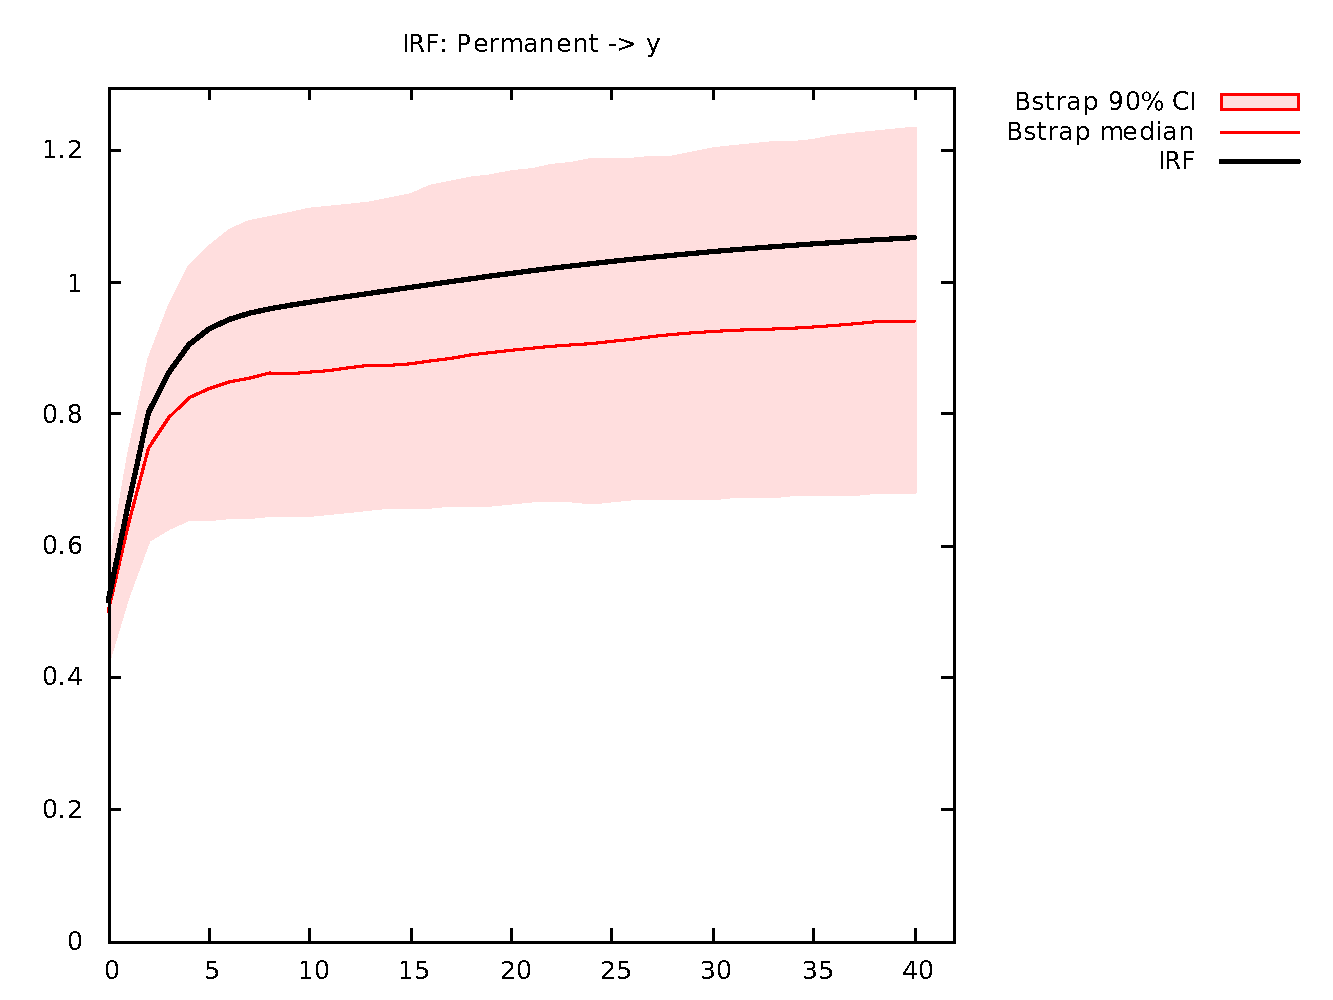
\includegraphics[height=4.75cm]{awm-irfy}
  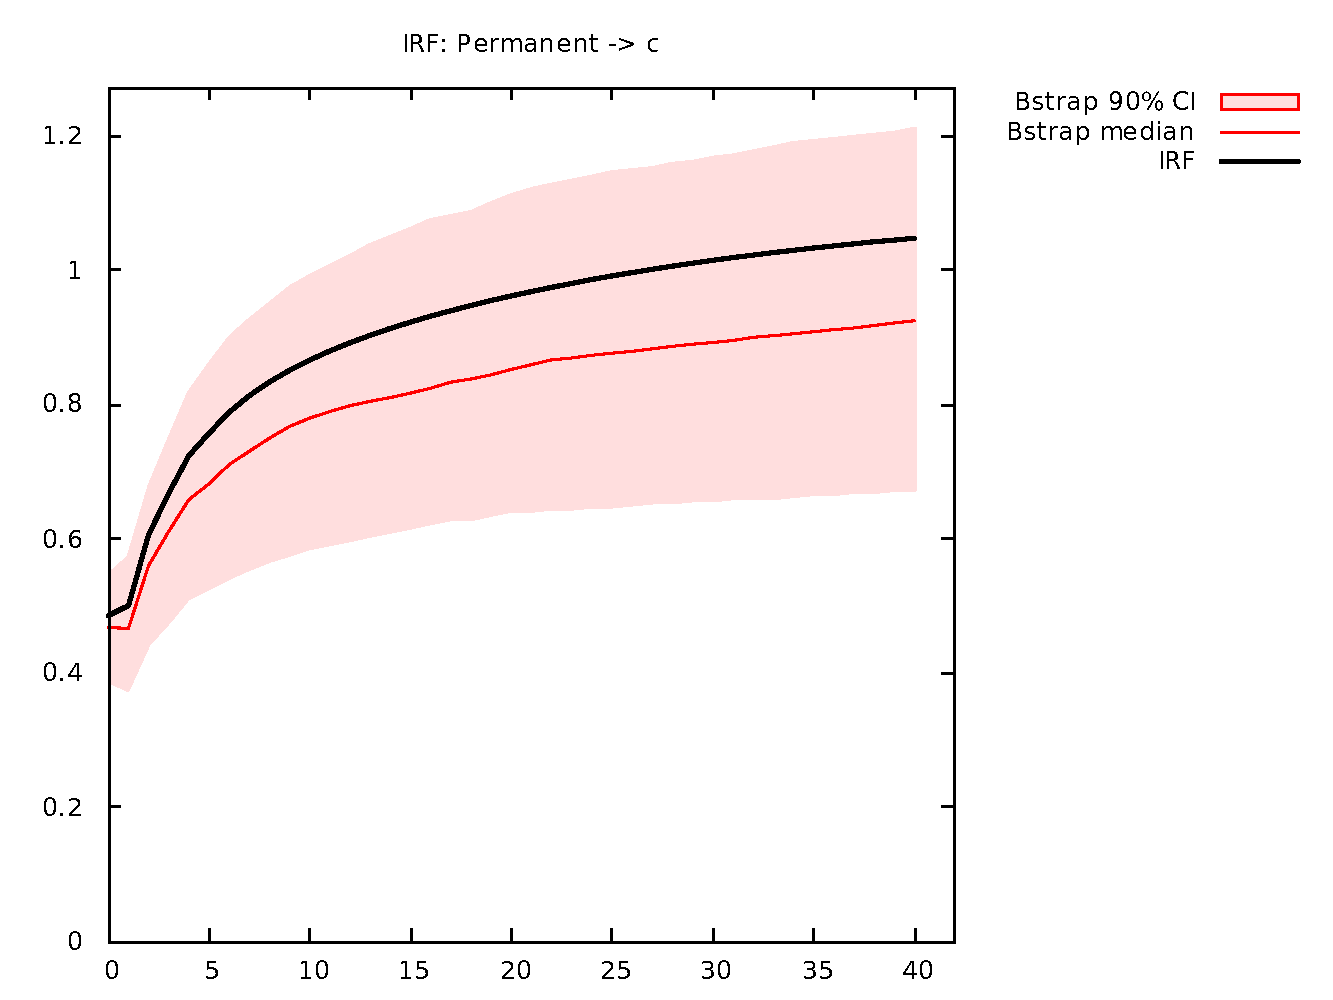
\includegraphics[height=4.75cm]{awm-irfc}
  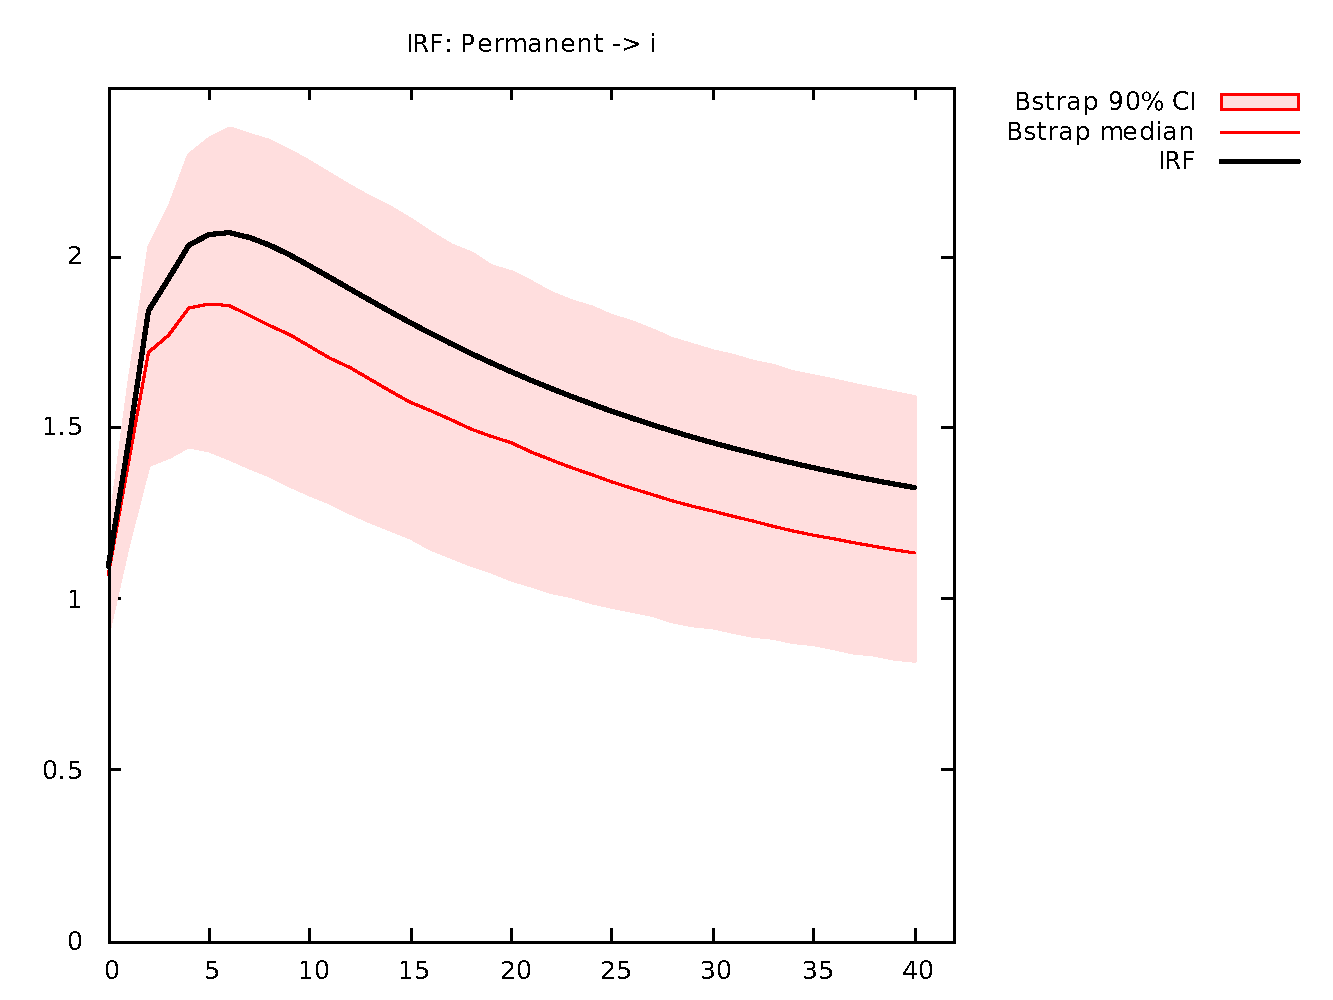
\includegraphics[height=4.75cm]{awm-irfi}
  \caption{Impulse responses to a permanent shock}
  \label{fig:AWM-irfs}
\end{figure}

More in detail, the script goes like this:
\begin{description}
\item[Lines 1--7] Create an empty quarterly dataset, populate it with
  the relevant variables from the \texttt{AWM.gdt} file.
\item[lines 8--13] Transform the series to logarithms and group them
  into the list \texttt{X}.
\item[lines 14--30] Run some preliminary checks: find the best lag
  length for the VAR, check that the cointegration rank is in fact 2
  and that the cointegration matrix is the one hypothesised by
  economic theory.
\item[Line 32] Set up the SVAR object. Note the usage of the
  \texttt{KPSW} code.
\item[Lines 33--36] Set up the cointegration infrastructure
  (deterministic terms, $\beta$, etcetera).
\item[lines 35--36] Set the horizon for IRF computation to a higher
  value than the default and add an extra restriction to one of the
  temporary shocks to achieve identification. Here we assume that the
  idiosyncratic shock on investment does not affect consumption
  instantaneously.
\item[lines 38--42] Estimate the model and plot the FEVD graphs.
\item[lines 43--46] Bootstrap the model and plot the IRFs with a
  90\% confidence interval.
\end{description}

A selection of the output is shown below, while Figure
\ref{fig:AWM-irfs} is the equivalent of \citeauthor{KPSW91}'s figure 2
(p. 820).\footnote{Note the usage of the fourth, optional parameter in
  the call to IRFplot to move the legend to the bottom of the figure.}
Considering that the data span a different period and describe a
different economy, the similarity between the original figure and the
replicated one is quite remarkable.

\begin{code}
# ok, now go for the real thing
? x = SVAR_setup("KPSW", X, const, p)
? matrix b = I(2) | -ones(1,2)
Generated matrix b
? SVAR_coint(&x, 3, b, {}, 1)
Unestricted constant, beta =
  1.00000  0.00000
  0.00000  1.00000
 -1.00000 -1.00000

alpha is unrestricted
? x.horizon = 40
? SVAR_restrict(&x, "C", 1, 2, 0)
? SVAR_estimate(&x)

Unconstrained Sigma:
     0.29538     0.39670     0.22203
     0.39670     1.64419     0.55188
     0.22203     0.55188     0.32538

C1 (3 x 3)

     0.97501      0.31359      0.55519 
     0.97501      0.31359      0.55519 
     0.97501      0.31359      0.55519 

Optimization method = Scoring algorithm

             coefficient   std. error      z       p-value 
  ---------------------------------------------------------
  C[ 1; 1]     0.485389    0.0391266     12.41     2.44e-35 ***
  C[ 2; 1]     1.09533     0.0948831     11.54     7.92e-31 ***
  C[ 3; 1]     0.516670    0.0406739     12.70     5.71e-37 ***
  C[ 1; 2]     0.00000     0.00000       NA       NA       
  C[ 2; 2]     0.373888    0.0245469     15.23     2.18e-52 ***
  C[ 3; 2]    -0.211184    0.0138649    -15.23     2.18e-52 ***
  C[ 1; 3]     0.244504    0.0160525     15.23     2.18e-52 ***
  C[ 2; 3]    -0.551965    0.0501828    -11.00     3.86e-28 ***
  C[ 3; 3]    -0.117619    0.0210737     -5.581    2.39e-08 ***

  Log-likelihood = -295.974
\end{code}

%\pagebreak[4]

\bibliography{SVAR}

\appendix

\pagebreak

\section{The GUI interface}
\label{sec:GUI}

\emph{by Sven Schreiber}

\vfil 

This section introduces the GUI interface with which most of the
available calculations can be accomplished as well and which can be
accessed via the \emph{Model $>$ Time Series $>$ Structural VAR} menu
entry of the the graphical \app{gretl} client.  While we recommend
using the script interface to access the full capabilities of the SVAR
package, the GUI interface may be less intimidating for less
experienced users. At the time of writing, the GUI component covers
everything but the SVEC case (see section \ref{sec:SVECs}) where the
cointegration properties of the system are exploited for special
long-run restrictions. The SVEC case will receive its own GUI in a
future version of the SVAR package. 

\begin{figure}[htbp]
  \centering
  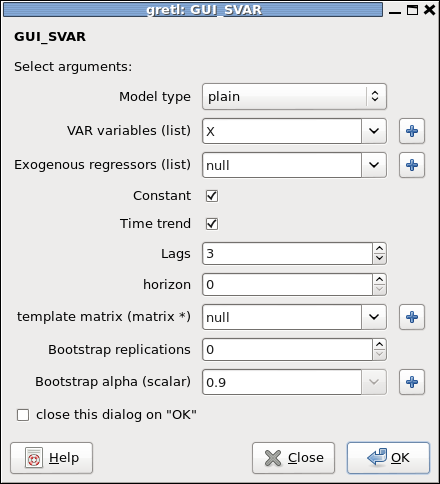
\includegraphics[scale=0.5]{GUI_SVAR.png}
  \caption{Plain Cholesky model through the GUI interface }
  \label{fig:GUI-plain}
\end{figure}


Many important contents of the window displayed in figure
\ref{fig:GUI-plain} should be rather self-explanatory; the model type
chooser, the list of endogenous VAR variables, another (optional) list
of exogenous variables, the lag order, and further down the number of
bootstrap replications along with the nominal bootstrap confidence
level (leave the number of replications at the default value zero to
skip the bootstrap), and finally the choice of the precise
optimization algorithm from the drop-down menu at the bottom, where as
before the scoring algorithm is the default.

The other function parameters will be explained now. First there are
three checkboxes that specify the deterministic terms to be included
in the model.\footnote{The seasonal dummies are automatically
  centered, which should only matter in the rather exotic case without
  a constant term, however.} Note that it is still possible to
manually specify the deterministic terms as in the script interface,
namely as part of the exogenous regressor list. Next, the
\emph{horizon} parameter sets the desired maximum impulse response
horizon as explained above for the script interface, and can be left
at zero to invoke the default settings.

\subsection{Identifying constraints}

The two central inputs for the C and AB model types are the
identifying constraints. In the SVAR GUI they must be given as pattern
matrices that can only have two types of entries: Each entry with a
"missing" value denotes an unrestricted element, and every entry with
a valid numerical value will be restricted to just that value. You can
either pre-define the pattern matrices before you call the SVAR
package and then choose the corresponding name of the matrix in the
drop-down menu, or you have to click on the ``+'' button next to the
function argument field and specify the matrix on the spot in the
following standard \app{gretl} matrix creation dialog.\footnote{Hint:
  with recent gretl versions it is possible to initialize the matrix
  to hold only missing values, by entering \texttt{na} or \texttt{nan}
  as the initial fill value. Then you just have to edit the actually
  restricted elements afterwards.} If you do not wish to restrict any
of the involved matrices, just leave the function argument at the
default "null" value.

For a C model, as indicated by the function argument labels the first
restriction pattern matrix refers to the short-run restrictions, while
the second pattern matrix must be used for the long-run
restrictions. If you choose an AB model instead, these matrix inputs
serve to hold the restrictions on B and A, respectively. Note the
reversed ordering of B and A here, which reflects the fact that if A
is the identity matrix then B is the same thing as the short-run
restriction C matrix, so these latter two matrices belong together.

\subsection{Bootstrap parameters and cumulation}

The next checkbox after the bootstrap specification concerns the
activation of the bias correction that was already explained in
relation to the script interface. Following is another checkbox that
activates a check for identification, see section \ref{sec:SVARid}.

Towards the end of the SVAR GUI window you have another matrix
argument which serves to tell the package which of the impulse
responses should be provided in cumulated form. You need to provide a
(row or column) vector that holds the corresponding integer indices of
the variables to be cumulated referring to the list of endogenous
variables. Say your list of endogenous variables is ``foo baz bar''
and the responses of \emph{foo} and \emph{bar} should be cumulated,
then you would need to pass a vector \texttt{\{1, 3\}} (or
\texttt{\{1; 3\}}).\footnote{This way of specifying the responses to
  be cumulated in the GUI of SVAR may change in the future, perhaps by
  using another list of variables instead.} Note that you can type an
expression of this sort into the matrix entry box directly, as shown in
Figure~\ref{fig:matrix-entry}.

\begin{figure}[htbp]
  \centering
  
\includegraphics[scale=0.5]{dialog_mat.png}
  \caption{Entering a matrix specification directly}
  \label{fig:matrix-entry}
\end{figure}

\subsection{The output window}

After specifying all necessary function arguments and clicking OK, you
are presented---possibly after having to wait for the CPU intensive
bootstrap to finish---with a first output window holding the basic
estimation results, for example of the C matrix or of the A and B
matrices. If the provided restrictions are over-identifying the
corresponding LR test result is also printed out.

In the SVAR output window (see Figure~\ref{fig:GUI-output} below)
three toolbar buttons deserve special mention: The ``Save'' button
allows you to save the printed output, but more importantly you can
also save the entire bundle that was returned by the SVAR package as
an icon (element) of the current \app{gretl} session. When you open
(view) the bundle again later, some information about the model
specification will also be shown. (And the session can in turn later
be saved into a session file.) Next, for saving only selected members
of the SVAR bundle there is the ``Save bundle content''
button. Finally you have the ``Graph'' button which provides the
access to the central SVAR analyses, namely the impulse responses, the
error variance as well as the historical decompositions.

\subsection{An example}

For example, suppose we wanted to estimate a C model like the one used
as example so far, with the only difference that we want the $C$
matrix to be \emph{upper} triangular, rather than lower
triangular. Via a script, you would use the function
\texttt{SVAR\_restrict()}, as in
\begin{code}
# Force C_{2,1} to 0
SVAR_restrict(&Mod, "C", 2, 1, 0)
\end{code}
but you can do the same via the GUI interface by using a pattern
matrix, which must be a $n \times n$ matrix (that is, the same
size as $C$). 

\begin{figure}[htbp]
  \centering
  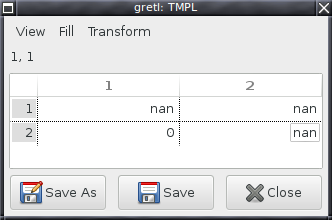
\includegraphics[scale=0.5]{TMPL.png}
  \caption{Template matrix}
  \label{fig:tmpl}
\end{figure}

Suppose we call the pattern matrix \texttt{TMPL} and that we select
the option ``Build Numerically'' (of course, with 2 rows and 2 columns
in this example).  When you're done, you return to the main SVAR
window (be sure to select C-model as the model type). After clicking
``OK'', the results window will appear, as in
Figure~\ref{fig:GUI-output}. Note that the estimated $C$ matrix is now
upper triangular.

From the output window, you can save the model bundle to the Icon view
by clicking on the leftmost icon\footnote{The visual appearance of the
  icons on your computer may be different from the one shown in Figure
  \ref{fig:tmpl}, as they depend on your software setup.  The number
  and ordering of the icons, however, should be the same on all
  systems.} and re-use it as needed for further processing.
\begin{figure}[htbp]
  \centering
  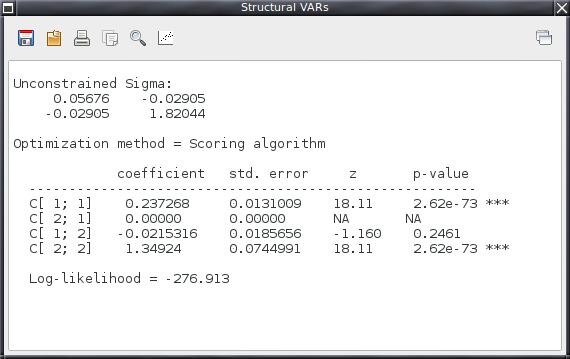
\includegraphics[scale=0.5]{Output.png}
  \caption{Output window}
  \label{fig:GUI-output}
\end{figure}

\clearpage

\section{Alphabetical list of functions}
\label{sec:syntax}

\begin{funcdoc}{FEVD(bundle *SVARobj)}
  Computes the Forecast Error Variance Decomposition from the
  structural IRFs, as contained in the model \texttt{SVARobj}. Returns
  an $h \times n^2$ matrix. The FEVD for variable $k$ is the block of
  columns from $(k-1) n + 1$ to $k n$ (where $n$ is the number of
  variables in the VAR).
\end{funcdoc}

\begin{funcdoc}{FEVDplot(bundle *obj, scalar vnum, int keypos[0:2:1])}
  Plots on screen the Forecast Error Variance Decomposition for a
  variable. Its arguments are:
  \begin{enumerate}
  \item a bundle holding the model
  \item the progressive number of the variable
  \item the position of the legend, if any (optional; default = right).
  \end{enumerate}
\end{funcdoc}

\begin{funcdoc}{FEVDsave(string outfilename, bundle *obj, scalar vnum, int keypos[0:2:1])}
  Saves the Forecast Error Variance Decomposition for a variable to a
  graphic file, whose format is identified by its extension. Its
  arguments are:
  \begin{enumerate}
  \item The graphic file name
  \item a bundle holding the model
  \item the progressive number of the variable
  \item the position of the legend, if any (optional; default = right).
  \end{enumerate}
\end{funcdoc}

\begin{funcdoc}{GetShock(bundle *SVARobj, scalar i)}
  Retrieves, as a series, the estimate of $i$-th structural shock of
  the system via equation \eqref{eq:PrE-StS-AB}, in which VAR
  residuals are used instead of the one-step-ahead prediction errors
  $\PrE{t}$. If the bundle \texttt{SVARobj} contains a non-null string
  \texttt{snames} with shock names, those are used in the description
  for the generated series.
\end{funcdoc}

\begin{funcdoc}{HDplot(bundle *obj, scalar vnum)}
  Plots on screen the Historical Decomposition for a variable. Its
  arguments are:
  \begin{enumerate}
  \item a bundle holding the model
  \item the progressive number of the variable
  \end{enumerate}
\end{funcdoc}

\begin{funcdoc}{HDsave(string outfilename, bundle *obj, scalar vnum)}
  Saves the Historical Decomposition for a variable to a graphic file,
  whose format is identified by its extension. Its arguments are:
  \begin{enumerate}
  \item The graphic file name
  \item a bundle holding the model
  \item the progressive number of the variable
  \end{enumerate}
\end{funcdoc}

\begin{funcdoc}{IRFplot(bundle *obj, scalar snum, scalar vnum, int keypos[0:2:1])}
  Plots an impulse response function on screen. Its arguments are:
  \begin{enumerate}
  \item a bundle holding the model
  \item the progressive number of the shock (may be negative, in which
    case the IRF is flipped)
  \item the progressive number of the variable
  \item the position of the legend, if any (optional; default = right).
  \end{enumerate}
\end{funcdoc}

\begin{funcdoc}{IRFsave(string outfilename, bundle *obj, scalar snum, scalar vnum, int keypos[0:2:1]))}
  Saves an impulse response function to a graphic file, whose format is
  identified by its extension. Its arguments are:
  \begin{enumerate}
  \item The graphic file name
  \item a bundle holding the model
  \item the progressive number of the shock (may be negative, in which
    case the IRF is flipped)
  \item the progressive number of the variable
  \end{enumerate}
\end{funcdoc}

\begin{funcdoc}{SVAR\_boot(bundle *obj, scalar rep, scalar alpha)}
  Perform a bootstrap analysis of a model. Returns the number of
  bootstrap replications in which the model failed to converge. Its
  arguments are:
  \begin{enumerate}
  \item a bundle holding the model
  \item the number of bootstrap replications
  \item the quantile used for the confidence bands
  \end{enumerate}
\end{funcdoc}

\begin{funcdoc}{SVAR\_coint(bundle *obj, scalar case,
			   matrix jbeta, matrix jalpha,
			   bool verbose[0])}
  Sets up a KPSW model for subsequent estimation. Its arguments are:
  \begin{enumerate}
  \item a bundle holding the model
  \item a code for the constant/trend combination (1 to 5, as per
    Johansen)
  \item the cointegration matrix (required)
  \item the loading matrix (optional, will be estimated via OLS if empty)
  \item an optional verbosity switch (default 0)
  \end{enumerate}
\end{funcdoc}


\begin{funcdoc}{SVAR\_cumulate(bundle *b, scalar nv)}
  Stores into the model the fact that the cumulated IRFs for
  variable \texttt{nv} are desired. This is typically used jointly
  with long-run restrictions.
\end{funcdoc}

\begin{funcdoc}{SVAR\_estimate(bundle *obj, int quiet)}
  Estimates the model by maximum likelihood. Its second argument is a
  scalar, which controls the verbosity of output. If omitted,
  estimation proceeds silently.
\end{funcdoc}

\begin{funcdoc}{SVAR\_hd(bundle *b, scalar nv)}
  Performs the ``historical decomposition'' of variable \texttt{nv}:
  this function outputs a list of variables which decomposes the
  \verb|nv|-th variable in the system into a deterministic component
  and $n$ stochastic components. The names of the resulting series are
  as follows: if the name of the decomposed variable is \texttt{foo},
  then the historical component attributable to the first structural
  shock is called \texttt{hd\_foo\_1}, the one attributable to the
  second structural shock is called \texttt{hd\_foo\_2}, and so
  on. Finally, the one for the first deterministic component is called
  \texttt{hd\_foo\_det}.
\end{funcdoc}

\begin{funcdoc}{SVAR\_ident(bundle *b, int verbose[0])}
  Checks if a model is identified by applying the algorithm described
  in \cite{AG}. Returns a 0/1 scalar. Its second argument is a
  scalar, which controls the verbosity of output. If set to a non-zero
  value, a few messages are printed as checks are performed.
\end{funcdoc}

\begin{funcdoc}{SVAR\_restrict(bundle *b, string code, scalar r, scalar c, scalar d)}
Sets up constraints for an existing model. The function which takes at
most five arguments:
\begin{enumerate}
\item A pointer to the model for which we want to set up the
  restriction(s)
\item A code for which type of restriction we want: 
  \begin{description}
  \item[\texttt{"C"}] Applicable to C models. Used for short-run
    restrictions.
  \item[\texttt{"lrC"}] Applicable to C models. Used for long-run
    restrictions.
  \item[\texttt{"A"}] Applicable to AB models. Used for constraints on
    the $A$ matrix.
  \item[\texttt{"B"}] Applicable to AB models. Used for constraints on
    the $B$ matrix.
  \item[\texttt{"Adiag"}] Applicable to AB models. Used for constraints on
    the whole diagonal of the $A$ matrix (see below).
  \item[\texttt{"Bdiag"}] Applicable to AB models. Used for constraints on
    the whole diagonal of the $B$ matrix (see below).
  \end{description}
\item An integer:
  \begin{description}
  \item[case 1]: applies to the codes \texttt{"C"}, \texttt{"lrC"},
    \texttt{"A"} and \texttt{"B"}. Indicates the row of the restricted element.
  \item[case 2]: applies to the codes \texttt{"Adiag"} and
    \texttt{"Bdiag"}. Indicates what kind of restriction is to be
    placed on the diagonal: any valid scalar indicates that the
    diagonal of $A$ (or $B$) is set to that value. Almost invariably,
    this is used with the value 1. IMPORTANT: if this argument is
    \texttt{NA}, all \emph{non-diagonal} elements are constrained to
    0, while diagonal elements are left unrestricted.
  \end{description}
\item An integer: the column of the restricted element, for the codes
  \texttt{"C"}, \texttt{"lrC"}, \texttt{"A"} and
  \texttt{"B"}. Otherwise, unused.
\item A scalar: for the codes \texttt{"C"}, \texttt{"lrC"},
  \texttt{"A"} and \texttt{"B"}, the fixed value the matrix element
  should be set to (may be omitted if 0). Otherwise, unused.
\end{enumerate}

A few examples: 
\begin{itemize}
\item \texttt{SVAR\_restrict(\&M, "C", 3, 2, 0)}; in a C model called
  \texttt{M}, sets $C_{3,2} = 0$. As a consequence, the IRF for
  variable number 3 with respect to the shock number 2 starts from
  zero.
\item \texttt{SVAR\_restrict(\&foo, "A", 1, 2, 0)}; in an AB model called
  \texttt{foo}, sets $A_{1,2} = 0$.
\item \texttt{SVAR\_restrict(\&MyMod, "lrC", 5, 3, 0)}; in a C model
  called \texttt{MyMod}, restricts $C$ such that the long-run impact
  of shock number 3 on variable number 5 is 0. This implies that the
  cumulated IRF for variable 5 with respect to shock 3 tends to zero.
\item \texttt{SVAR\_restrict(\&bar, "Adiag", 1)}; in an AB model called
  \texttt{bar}, sets $A_{i,i} = 1$ for $1 \le i \le n$.
\item \texttt{SVAR\_restrict(\&baz, "Bdiag", NA)}; in an AB model called
  \texttt{baz}, sets $B_{i,j} = 0$ for $i \ne j$.
\end{itemize}

If the restrictions are found to conflict with other ones already
implied by the pre-existing constraints, they will just be ignored and
a warning will be printed.
\end{funcdoc}

\begin{funcdoc}{SVAR\_setup(string type, list Y, list X, int varorder)}
  Initialises a model: the function's output is a bundle. The function
  arguments are:
  \begin{enumerate}
  \item A type string: at the moment, valid values are \texttt{"C"},
    \texttt{"plain"} and \texttt{"AB"};
  \item a list containing the endogenous variables;
  \item a list containing the exogenous variables;
  \item a positive integer, the VAR order.
  \end{enumerate}
\end{funcdoc}

\section{Contents of the model bundle}
\label{sec:bundle_struct}

  \centering
  \begin{tabular}{rp{0.8\textwidth}}
    \hline
    \multicolumn{2}{c}{\textbf{Basic setup}} \\
    \hline
    \texttt{step} & done so far \\
    \texttt{type} & string, model type \\
    \texttt{n}	  & number of endogenous variables \\
    \texttt{p}	  & VAR order \\
    \texttt{k}	  & number of exogenous variables \\
    \texttt{T}	  & number of observations \\
    \texttt{t1, t2}	  & initial and final observations \\
    \texttt{X}	  & exogenous variables data matrix \\
    \hline
    \multicolumn{2}{c}{\textbf{VAR}} \\
    \hline
    \texttt{VARpar} & autoregressive parameters \\
    \texttt{mu}	    & coefficients for the deterministic terms \\
    \texttt{E}	    & residuals from base VAR (as matrix) \\
    \texttt{Sigma}  & unrestricted covariance matrix \\
    \texttt{jalpha} & (SVEC only) cointegration loadings \\
    \texttt{jbeta}  & (SVEC only) cointegration coefficients \\
    \hline
    \multicolumn{2}{c}{\textbf{SVAR setup}} \\
    \hline
    \texttt{Rd1}	 & short-run constraints on B (and therefore C in non-AB models) \\
    \texttt{Rd1l}	 & long-run constraints on B (and therefore C in non-AB models) \\
    \texttt{Rd0}	 & contains short-run constraints on A in AB models \\
    \texttt{horizon}	 & horizon for structural VMA \\
    \texttt{cumul}	 & vector of cumuland variables \\
    \texttt{ncumul}	 & number of cumuland variables \\
    \texttt{Ynames}	 & string array, names for VAR variables \\
    \texttt{Xnames}	 & string array, names for exogenous
    variables, if any \\
    \texttt{snames}	 & string array, names for shocks \\
    \texttt{optmeth}	 & integer between 0 and 4, optimisation method \\
    \hline
    \multicolumn{2}{c}{\textbf{SVAR post-estimation}} \\
    \hline
    \texttt{S1}	   & estimated A (or C) \\
    \texttt{S2}	   & estimated B \\
    \texttt{theta} & coefficient vector \\
    \texttt{IRFs}  & IRF matrix (see section \ref{sec:baseest})\\
    \hline
    \multicolumn{2}{c}{\textbf{Bootstrap-related}} \\
    \hline
    \texttt{nboot}	 & number of bootstrap replications \\
    \texttt{boot\_alpha} & bootstrap confidence level \\
    \texttt{bootdata}	 & output from the bootstrap (see section \ref{sec:bootstrap})\\
    \texttt{biascorr}	 & scalar, 0 for no bias correction, 1 for
    partial, 2 for full
  \end{tabular}
\end{document}

%%% Local Variables: 
%%% mode: latex
%%% TeX-master: t
%%% End: 

